\newgeometry{textwidth=16cm}
\singlespacing
\chapter[Molecular dynamics study of the nano-aggregation in asphaltene]{Molecular dynamics study of the nano-aggregation in asphaltene mixtures: effects of the N, O and S heteroatoms}
\minitoc
\restoregeometry

\newpage


We present molecular dynamics simulations (MDS) for interpreting the molecular aggregation of:\footnote{\textit{Guevara Level et al. Energy \& Fuel, 30(6), 4758-4766, 2016}}
\begin{enumerate}
	\item \textit{six different asphaltene molecular models based on the C5Pe molecule;}
	\item \textit{several other derivatives based on the PA3 and CA22 structure issued from the recent work of isolation and identification of asphaltenes by Schuler \textit{et al.}\footnote{\textit{JACS}, \textbf{2015}, 137, 31, 9870}}
\end{enumerate}    

These simulations are based on recent X-ray (SAXS) and neutron (SANS) small-angle scattering experiments from Eyssautier \textit{et al.}\footnote{\textit{The J. of Phys. Chem. B}, \textbf{2011}, 115, 21, 6827} which proposed a discoidal asphaltene nanoaggregate structure of 0.67 nm height and its chemical composition. For the first topic, we have investigated the effect of sulfur atom position in the asphaltene structure and we have found that when it is grafted directly to the conjugated core no effect can be deducted from the stability of dimers and trimers and all the other studied parameters. This is not the case when sulfur is located in the lateral chain, where it has a particular affinity with oxygen and hydrogen atoms of the acid chain ends of neighbor molecules. Consequently, we suggest that these configurations of the sulfur atom are more likely to be problematic in oil industry. For the second topic, the chemical characteristics of these real asphaltene molecules were screened by changing the heteroatoms on the backbone and the lateral chain-ends. The results show that the interaction energies vary for different heteroatom arrangement within a given structure and depend on the type of asphaltene. Moreover, we showed that the chain-ends have a crucial role on this phenomenon.

\clearpage

\section{Introduction}

%%%%%%%%%%%%%%%%%%%%%%%%%%%%%%%%%%%%%%%%%%%%%%
%     À VOIR SI ÇA VAUT LA PEINE D'INCLURE CE MORCEAU CI-DESSOUS      %
%%%%%%%%%%%%%%%%%%%%%%%%%%%%%%%%%%%%%%%%%%%%%%

Asphaltenes are the oil's insoluble phase in light \textit{n}-alkanes and soluble in aromatic solvents like benzene or toluene\cite{mullins2011asphaltenes}. Their presence is critical and can cause problems in several fields of petroleum utilization, from oil recovery and transportation to refining.\cite{adams2014asphaltene} These complications arise from the tendency of asphaltenes to aggregate and form macro structures able to modify their flow properties (increasing oil viscosity, emulsion stability, etc.) and even, in the worst cases, stop the fluid production (plugging pores in the reservoir, well-bore tubing or flow-lines/pipelines, accumulating in separators, etc.) \cite{benamsili2013multi}.\\

Asphaltenes consist of a complex mixture of polycyclic aromatic hydrocarbons substituted with alkyl side chains. Carbon and hydrogen are the major atoms, but the molecules also contain heteroatoms, mainly sulfur.\cite{mullins2010modified} Although much knowledge has been gained throughout the last years, the molecular structure of this phase is poorly determined and can vary quite significantly depending on the origin, on the age of the crude oil and on the pressure and temperature conditions\cite{sabbah2011evidence}.\\

So, in order to fully understand their nature and to predict their structure, several analytical techniques have been used to gather information on their macromolecular structure. Small angle X-ray (SAXS) and neutron scattering (SANS) techniques have proved that the basics of their supramolecular arrangement is the discoidal $\pi$-stacking of the conjugated cores, with heights varying from 1 to 10 nm \cite{eyssautier2011insight,barre2009relation}.\\

From \textit{in silico} point of view, the study of asphaltene aggregation makes use of molecular dynamics simulations. Several force-fields have proved to produce results consistent with experimental results.\cite{sedghi2013effect,liu2015molecular,gao2014molecular} Thereby, we have, in a first moment, chosen six asphaltene molecular models, as dimers and trimers in toluene, to investigate the sulfur atom position in the structure and the consequent effect on the stability of dimers and trimers in solution. These models are based on the C5Pe model module, a prototypical asphaltene molecule that has been reported and used in several studies\cite{gao2014molecular,teklebrhan2014initial}.\\

Experimental work in progress using this molecule also justifies this choice that allows us to compare experience and theory. This work aims to investigate the influence of sulfur atoms on C5Pe's dimers and trimers stabilization during a 150 ns time-delay in toluene at 298K and 1 atm conditions. In this way, all the other possible parameters influencing the nano-aggregation of asphaltenes (size of conjugated core, lateral chains, etc...) are excluded and one can really screen the effect of sulfur atoms in this physical-chemical process.\\

Then, the first part of this study uses the N-(1-Hexylheptyl)-N'-(5-carboxy-licpentyl)-perylene-3,4,9,10-tetracarboxylicbisimide molecule (C5Pe, molecule 1) and three C5Pe analogues (molecules 2, 3, and 4), with the presence of sulfur atom at different positions (core and side chain) as test cases. Two other molecules, 5 and 6, respectively, were studied: the situation where all the \ce{C=O} groups are replaced by \ce{C=S} ones (the extreme of molecule 2) and the situation where no heteroatom is found in this position (\ce{C-H} bond, quinoid structure imposed). 

\begin{figure}[htb]
	\centering
	\begin{tabular}{cc}
		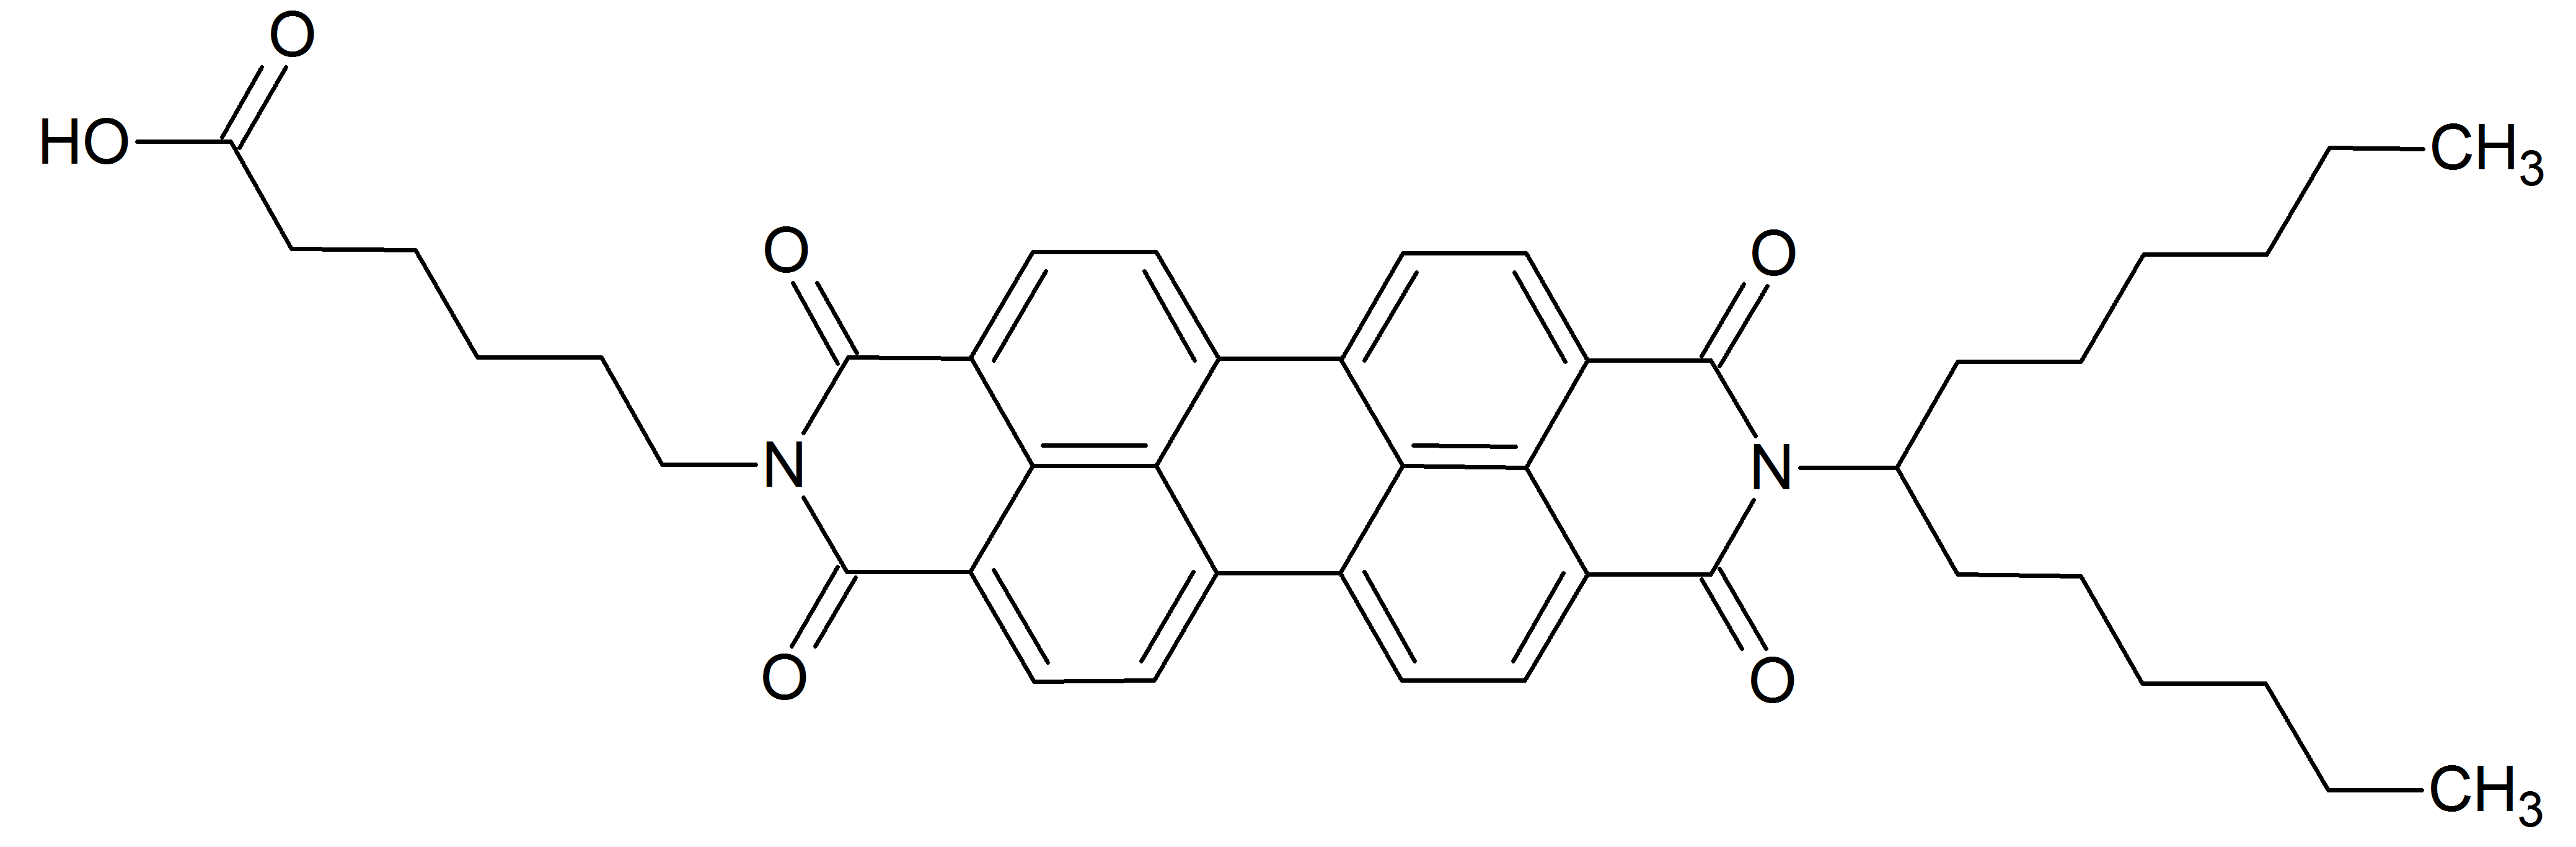
\includegraphics[width=0.45\columnwidth]{image/1} &
		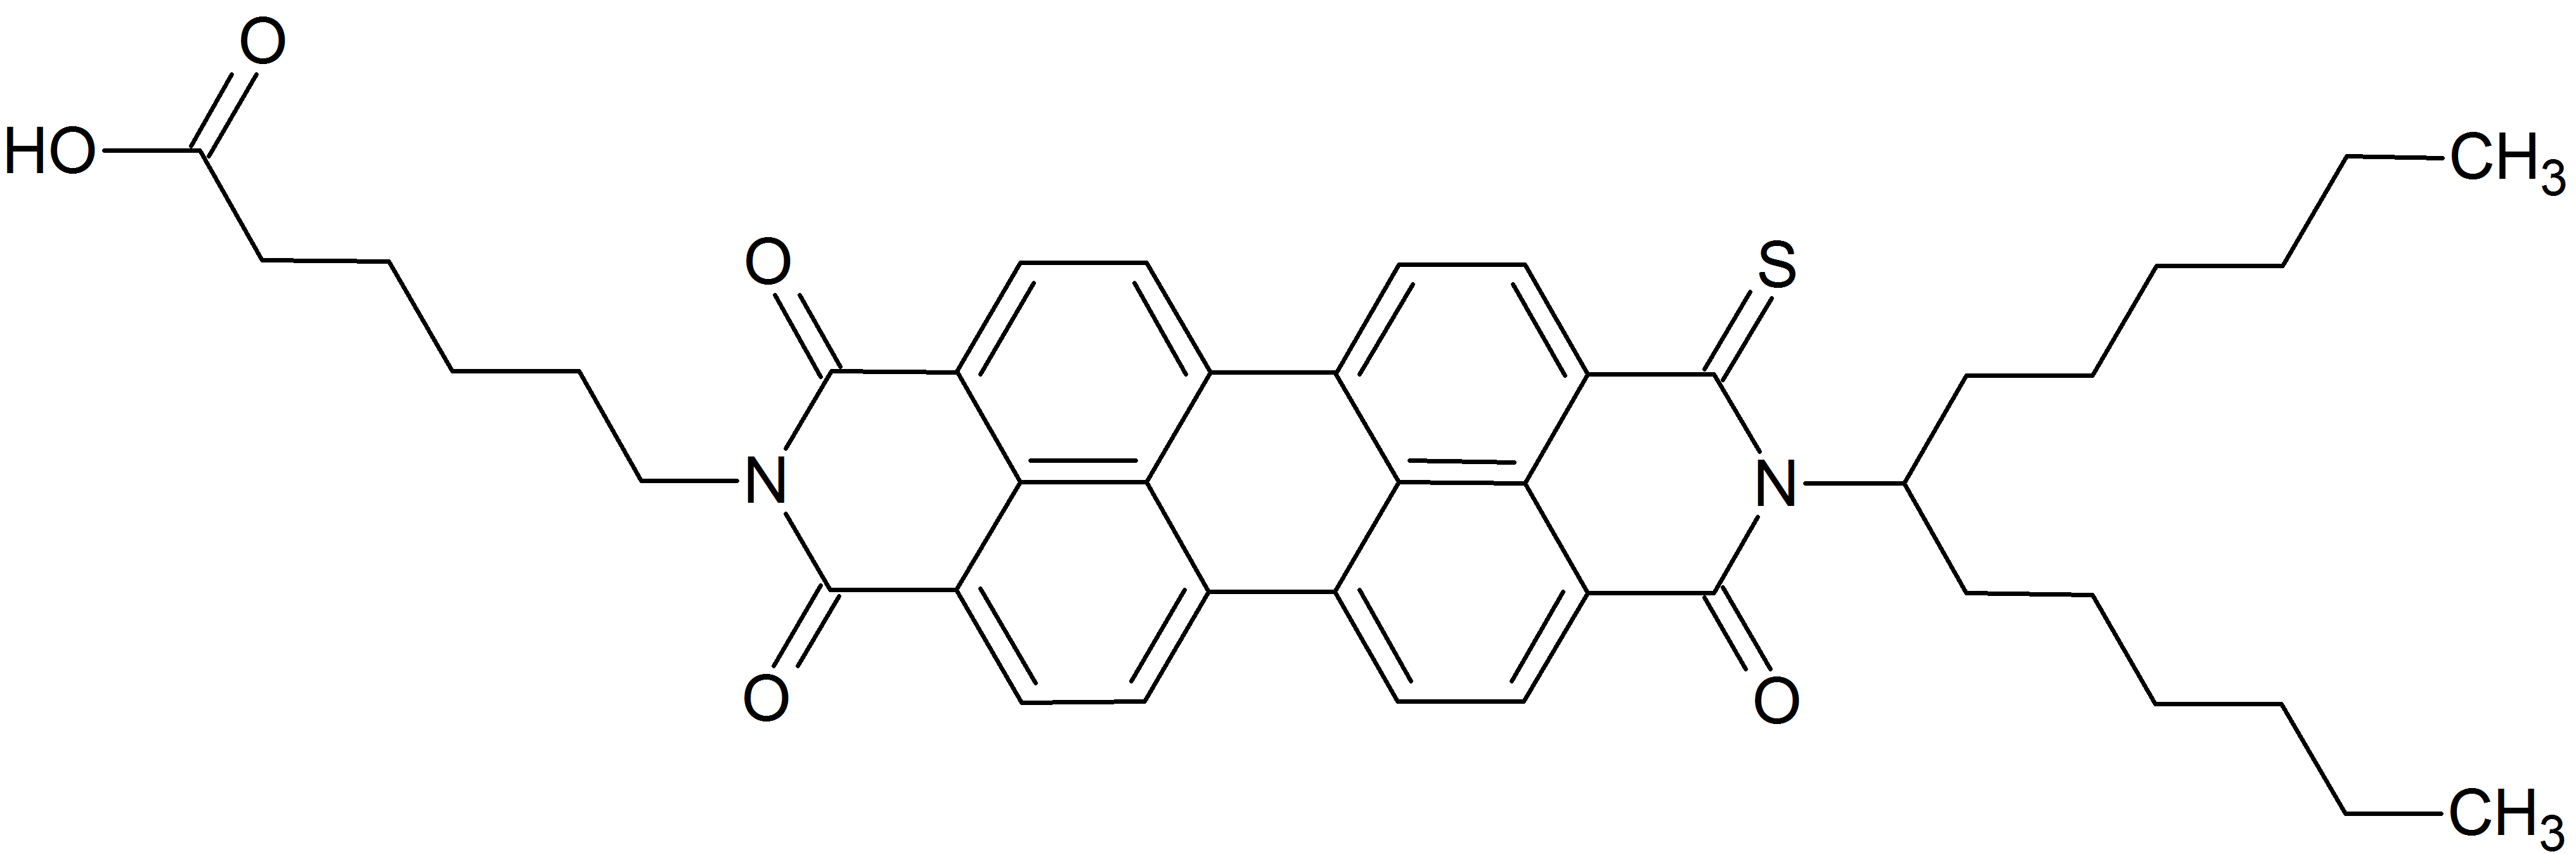
\includegraphics[width=0.45\columnwidth]{image/2}\\
		Molecule 1 & Molecule 2\\
		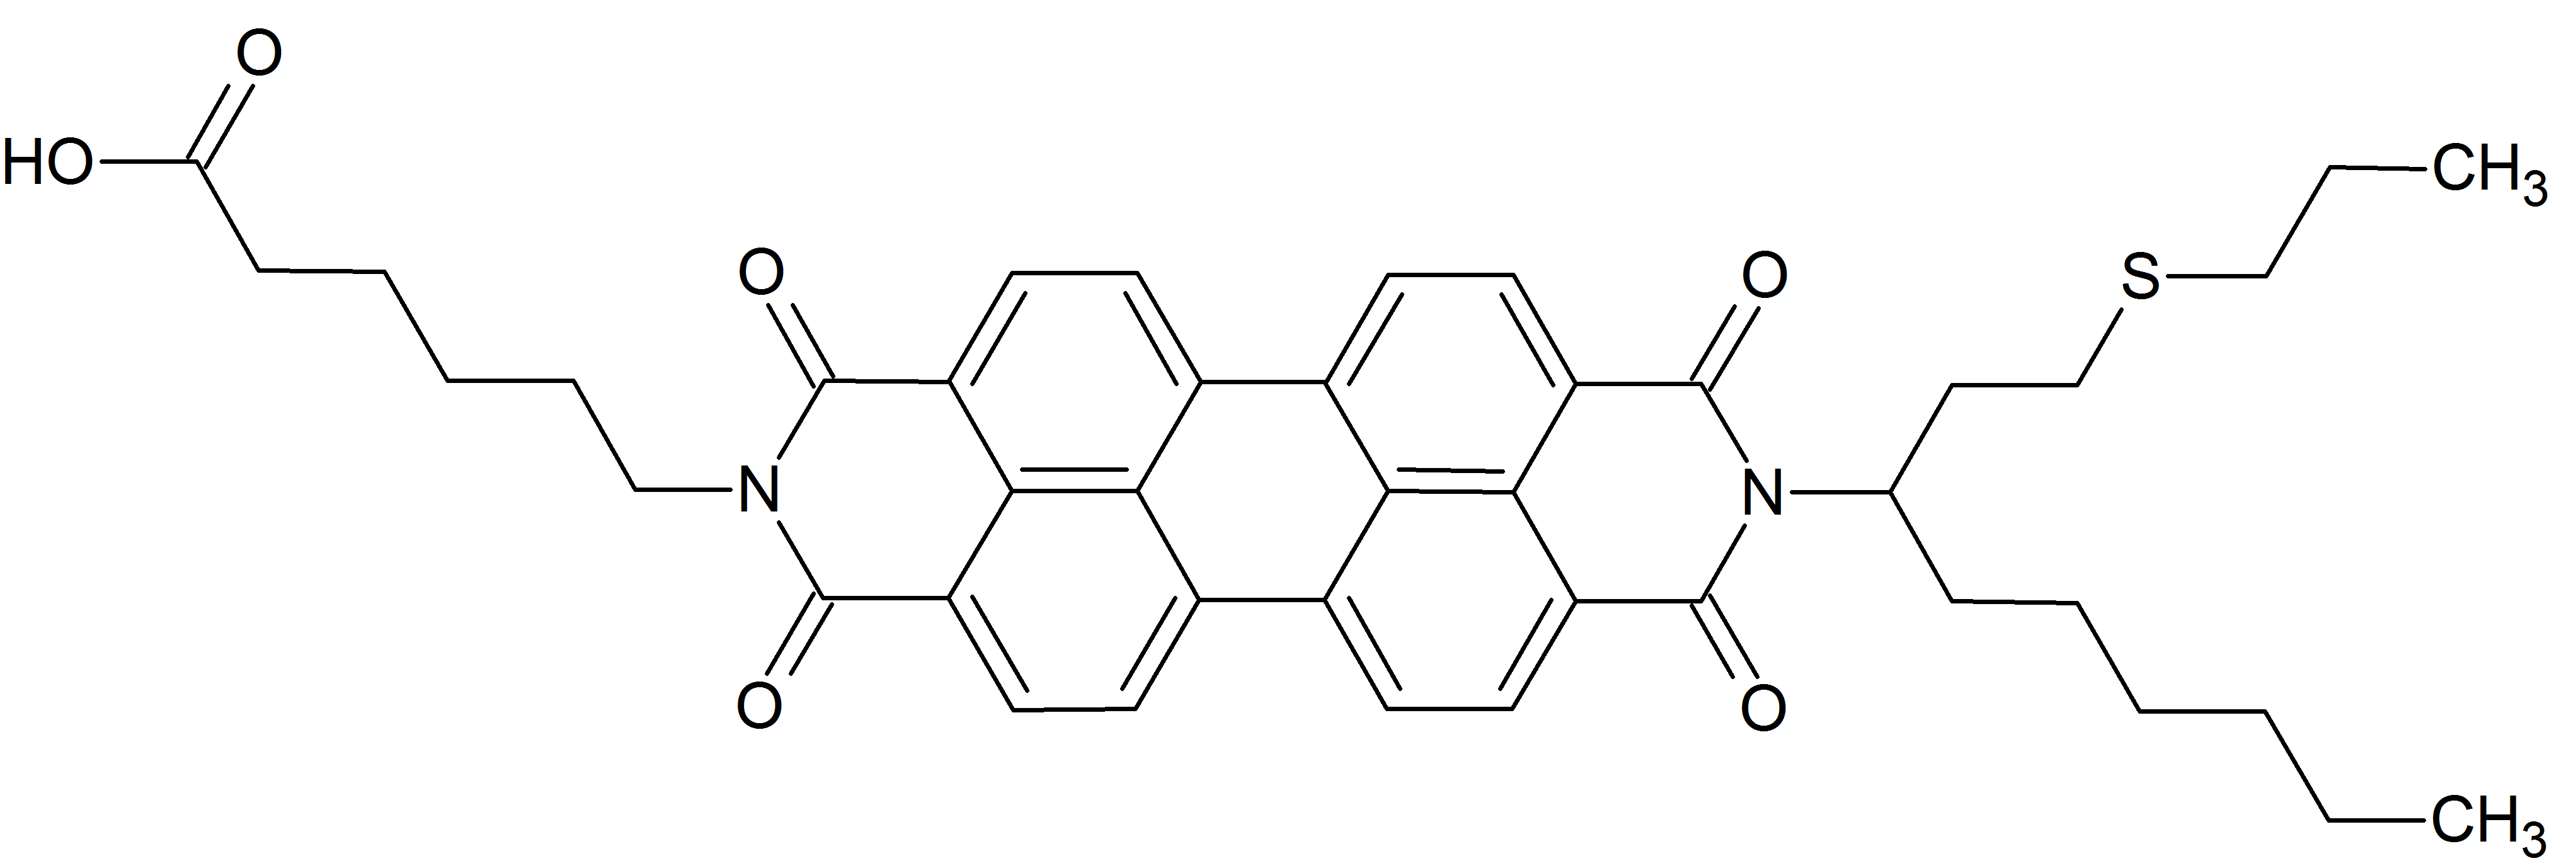
\includegraphics[width=0.45\columnwidth]{image/3} &
		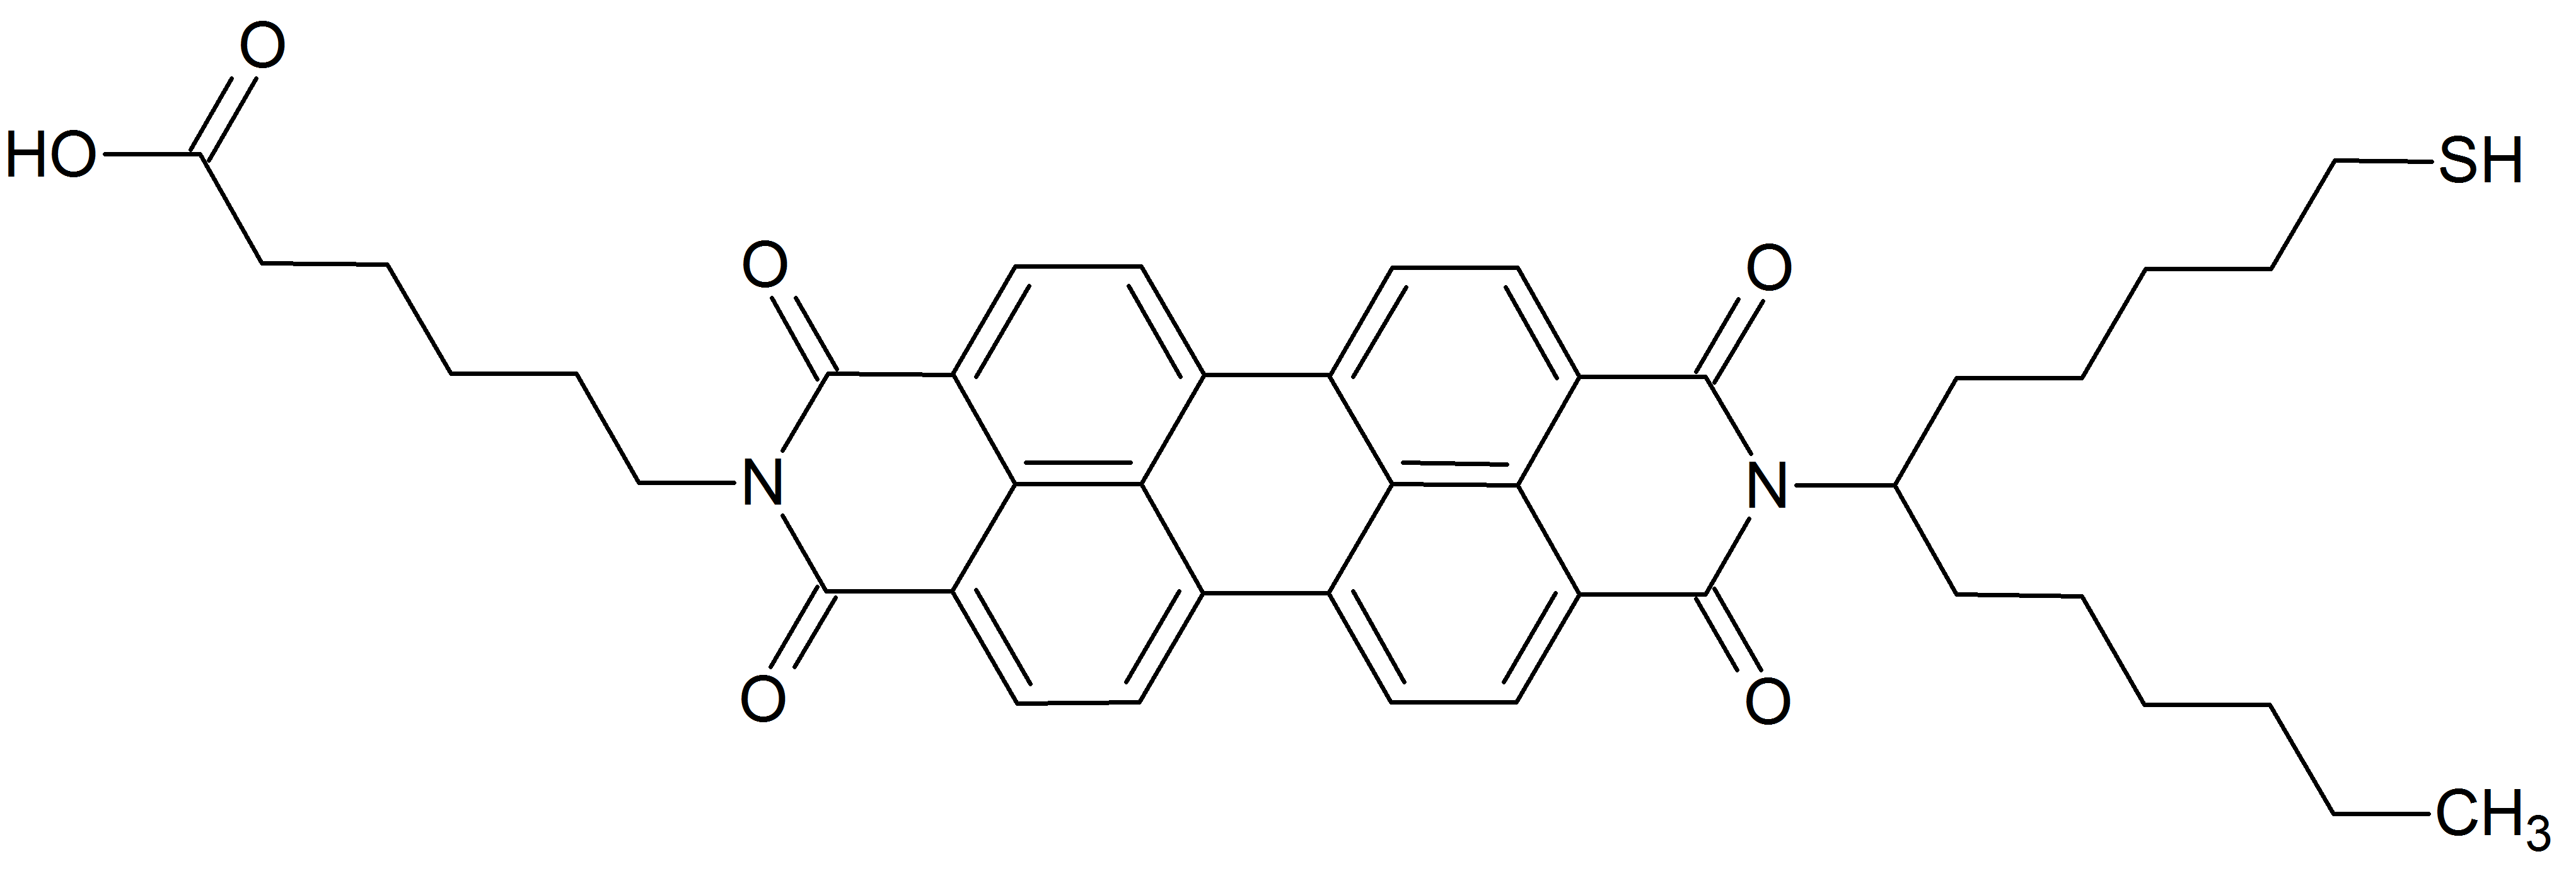
\includegraphics[width=0.45\columnwidth]{image/4}\\
		Molecule 3 & Molecule 4\\
		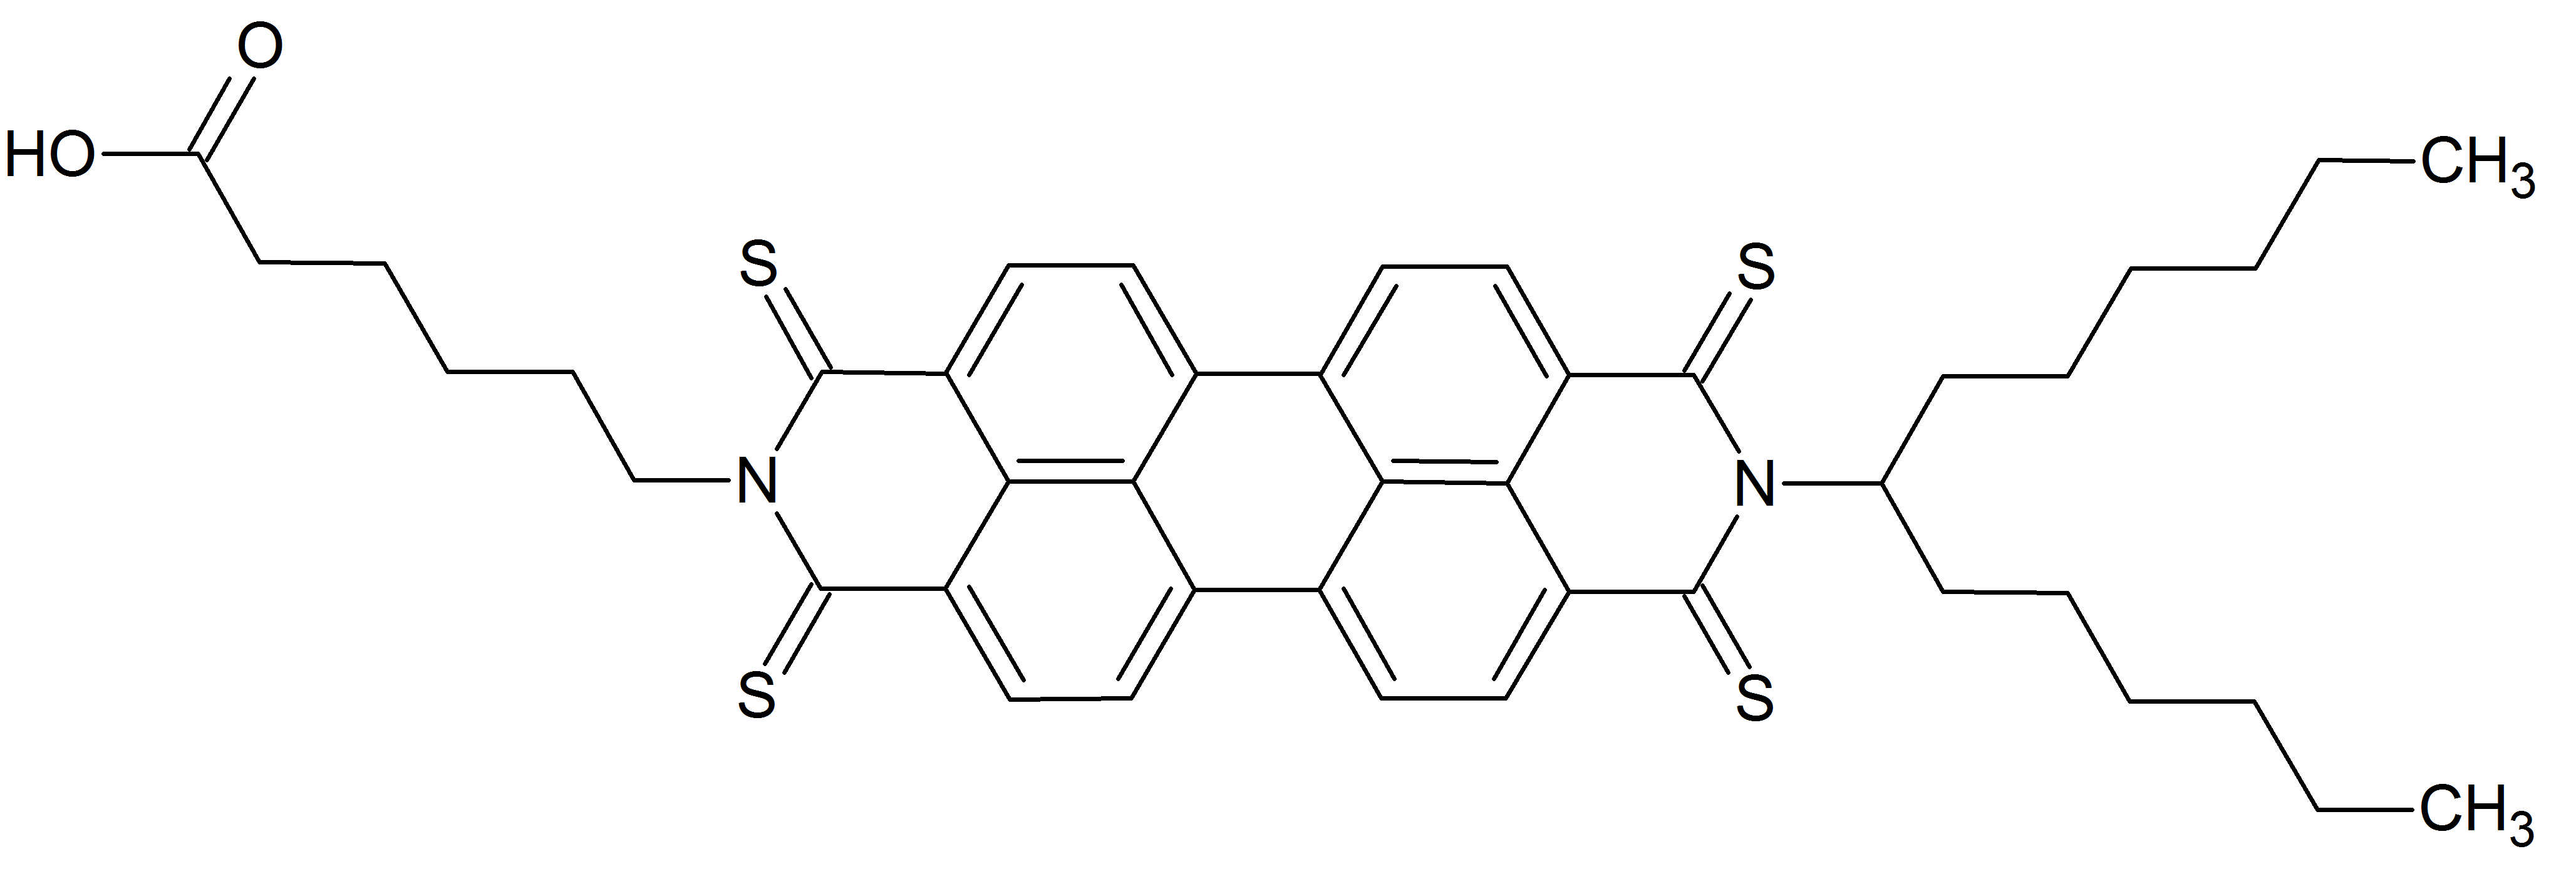
\includegraphics[width=0.45\columnwidth]{image/5} &
		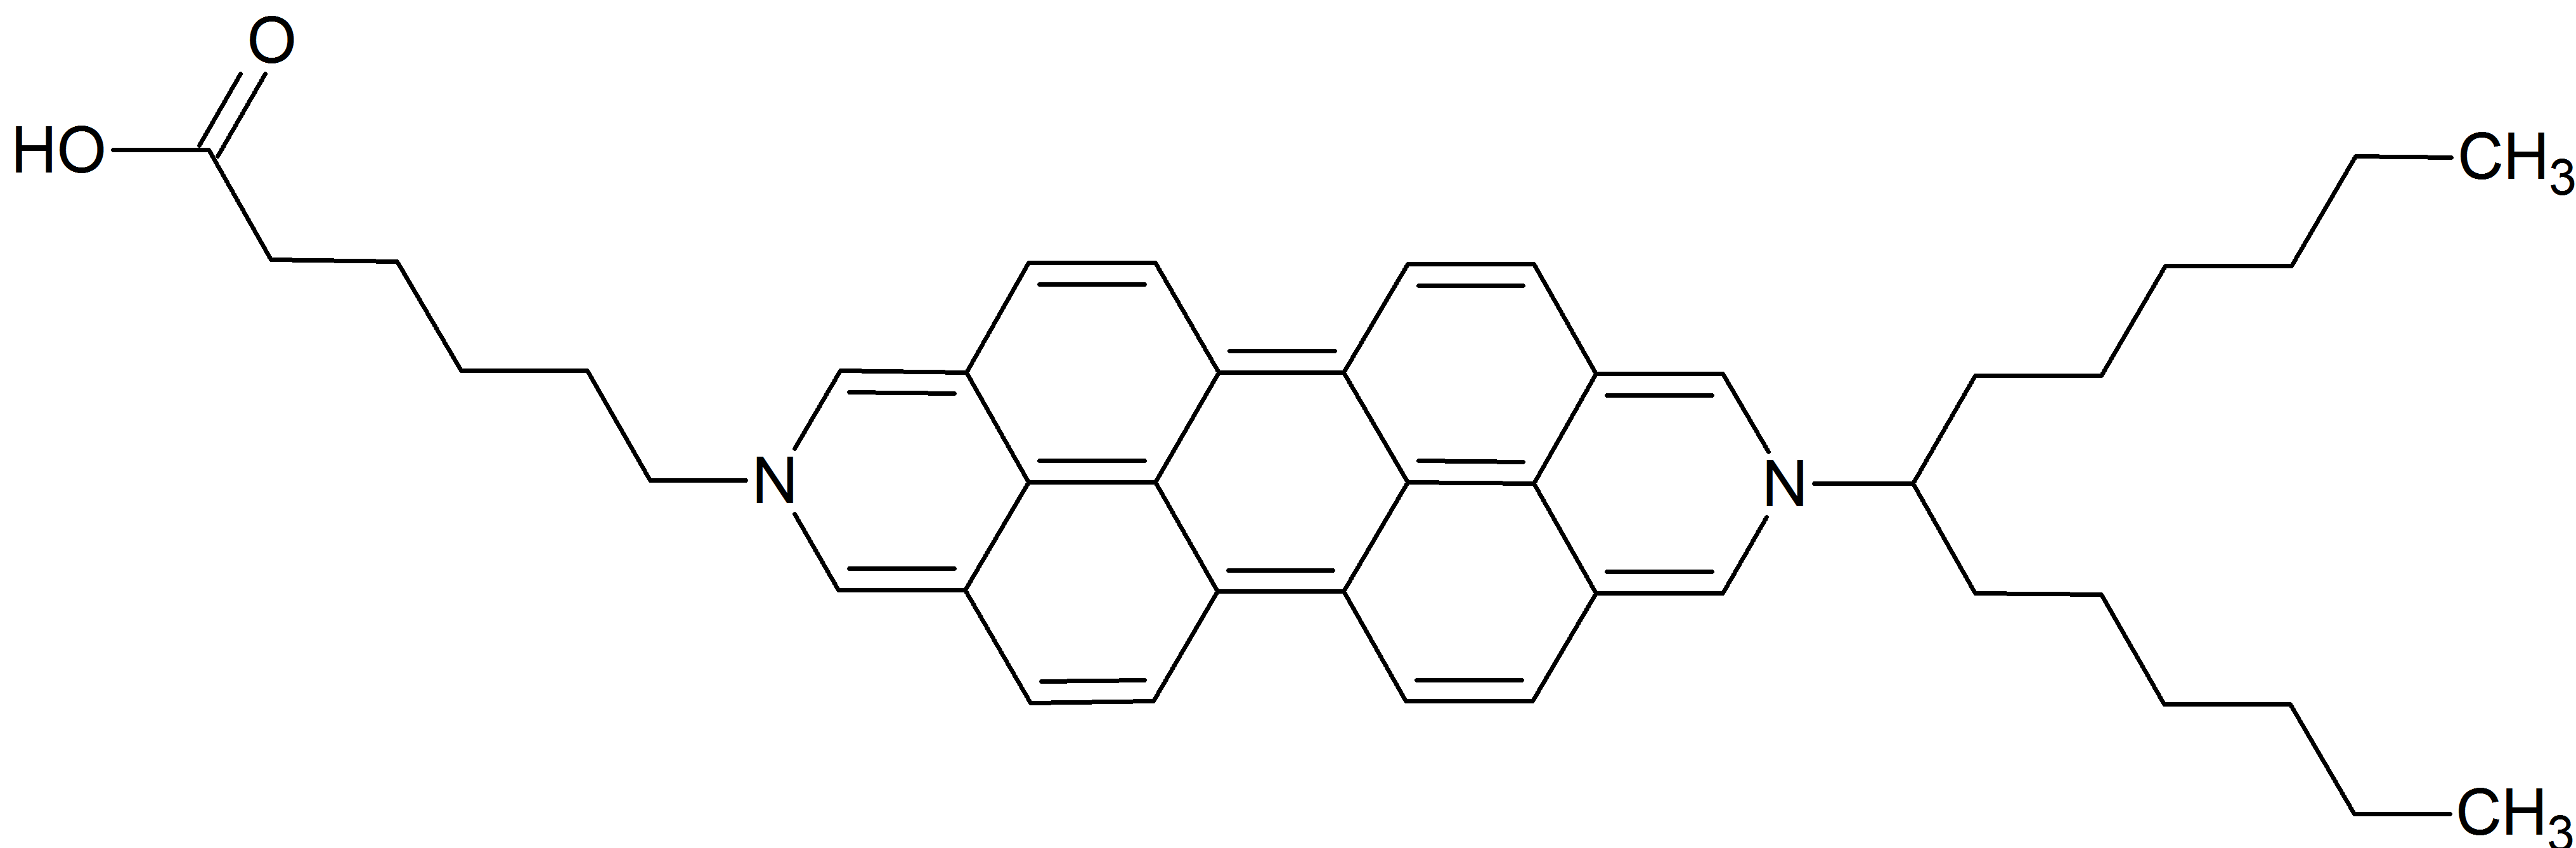
\includegraphics[width=0.45\columnwidth]{image/6}\\
		Molecule 5 & Molecule 6\\        
	\end{tabular}
	\caption{C5Pe molecular models of asphaltenes. }
	\label{pap:fig01}
\end{figure}

For each solvated asphaltene system using the C5Pe model, the initial configuration was constructed in a box with the 2 or 3 asphaltene molecules models. Two starting points were envisaged: 1) their poly-aromatic cores are anti-parallel to each other and the aggregate is already formed (this is called the``organized'' configuration); and 2), the molecules were randomly inserted in the simulation box. For the former case, the spacing between the mass centers of two neighboring asphaltene molecules is 0.35 nm in the -stacking direction. Finally, for both cases, the box was randomly filled with toluene molecules.\\

More recently, Schuler \textit{et al.}'s\cite{schuler2015unraveling} work brought more evidences on the molecular structures of asphaltenes based on Atomic Force Microscopy (AFM). They report the isolation of several distinct molecules which are in good agreement with the commonly accepted asphaltene structure: basically composed of aromatic cores, substituted by heteroatoms and presence of alkyl side chains with a variable number of carbons. We have chosen two among these molecules in order to study the effect of the heteroatom substitution on the conjugated aromatic core and the mixture in the crude oil and how the aggregation can occur in a more realistic model than just using one molecule at a time. The selected molecules, depicted in Figure \ref{pap:fig01}, are originally labeled PA3 and CA22 after Schuler \textit{et al.},\cite{schuler2015unraveling} both of them being of the continental type.\cite{mullins2010modified,mullins2011asphaltenes,mullins2012advances} Finally, it is worth saying that the CA22 molecule is a coal asphaltene rather than a petroleum asphaltene. It is herein used since it has a conjugated core size sensibly different from the PA3 one.

\begin{figure}[htb]
	\centering
	\begin{tabular}{cc}
		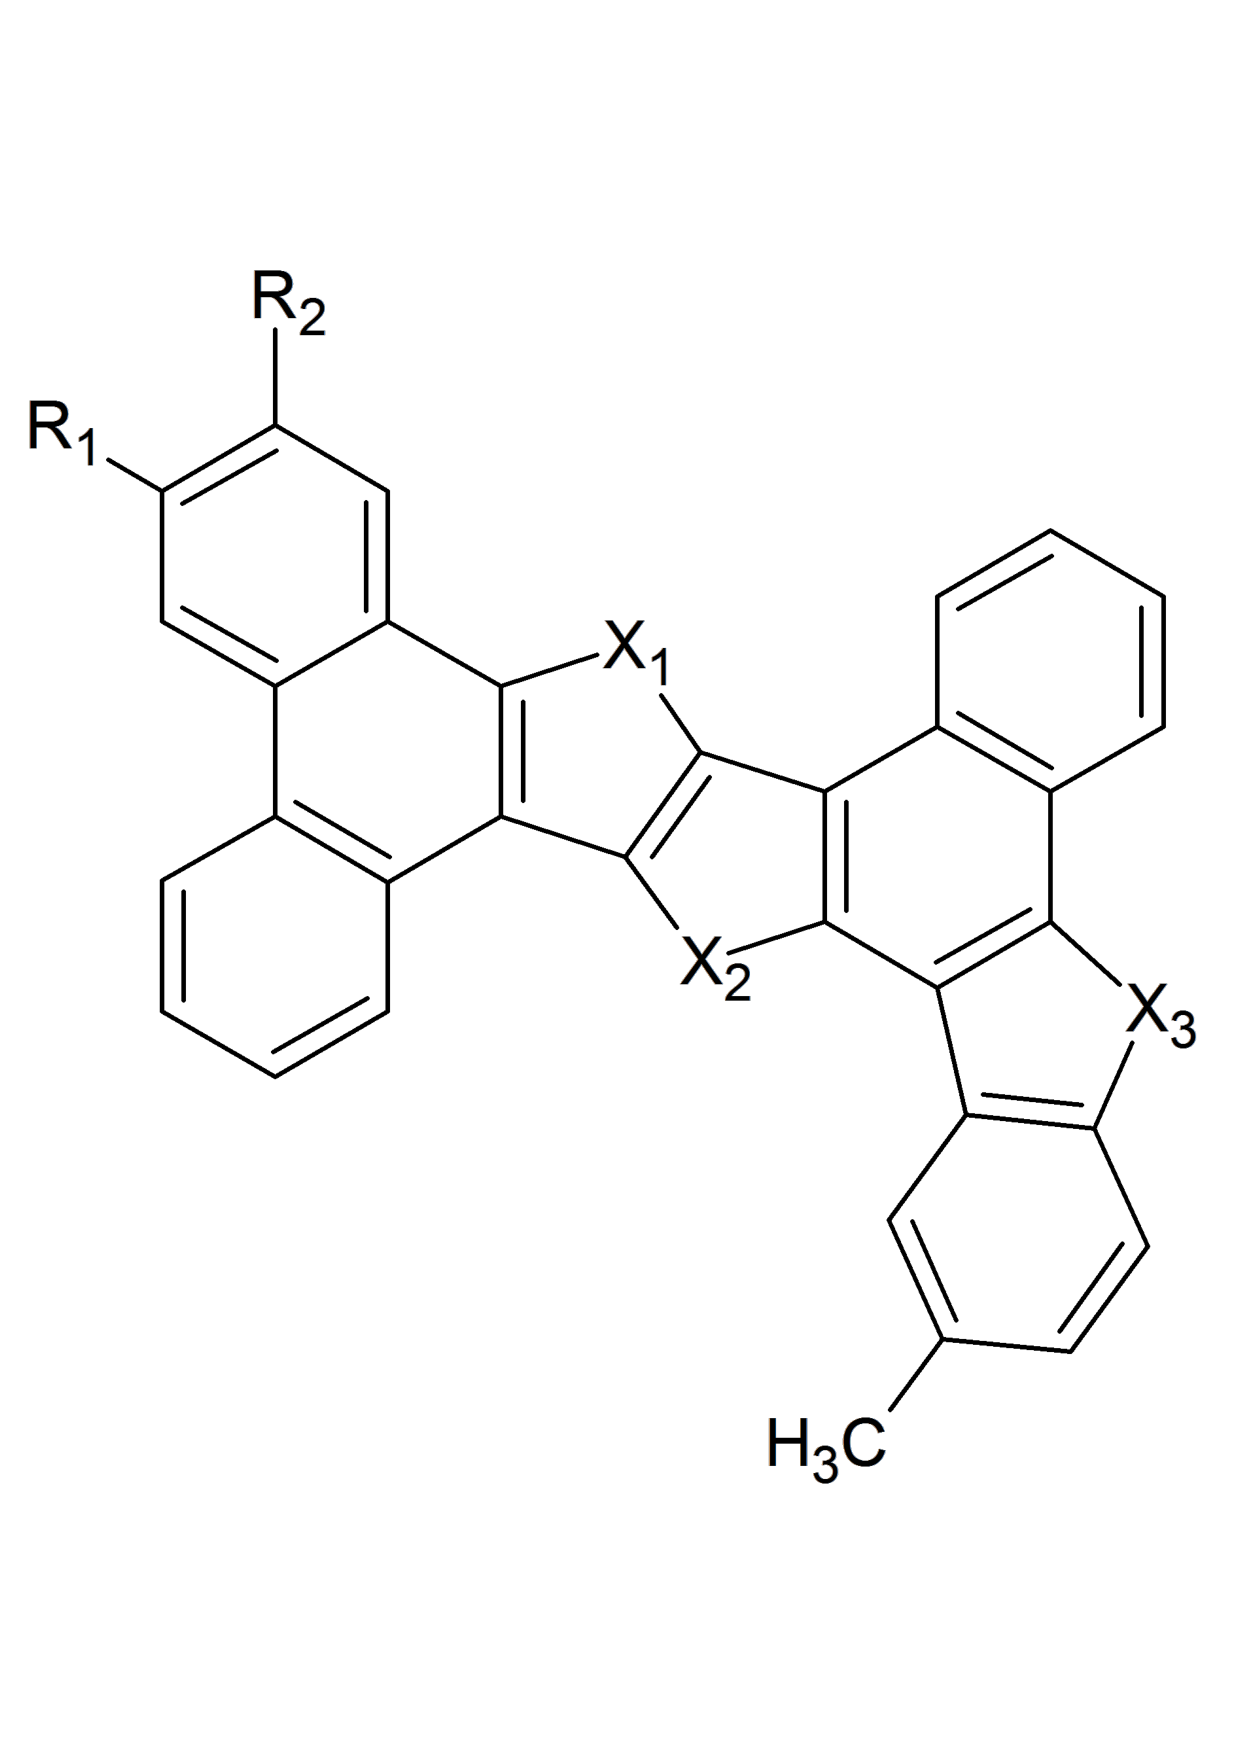
\includegraphics[width=0.35\columnwidth]{image/PA3} &
		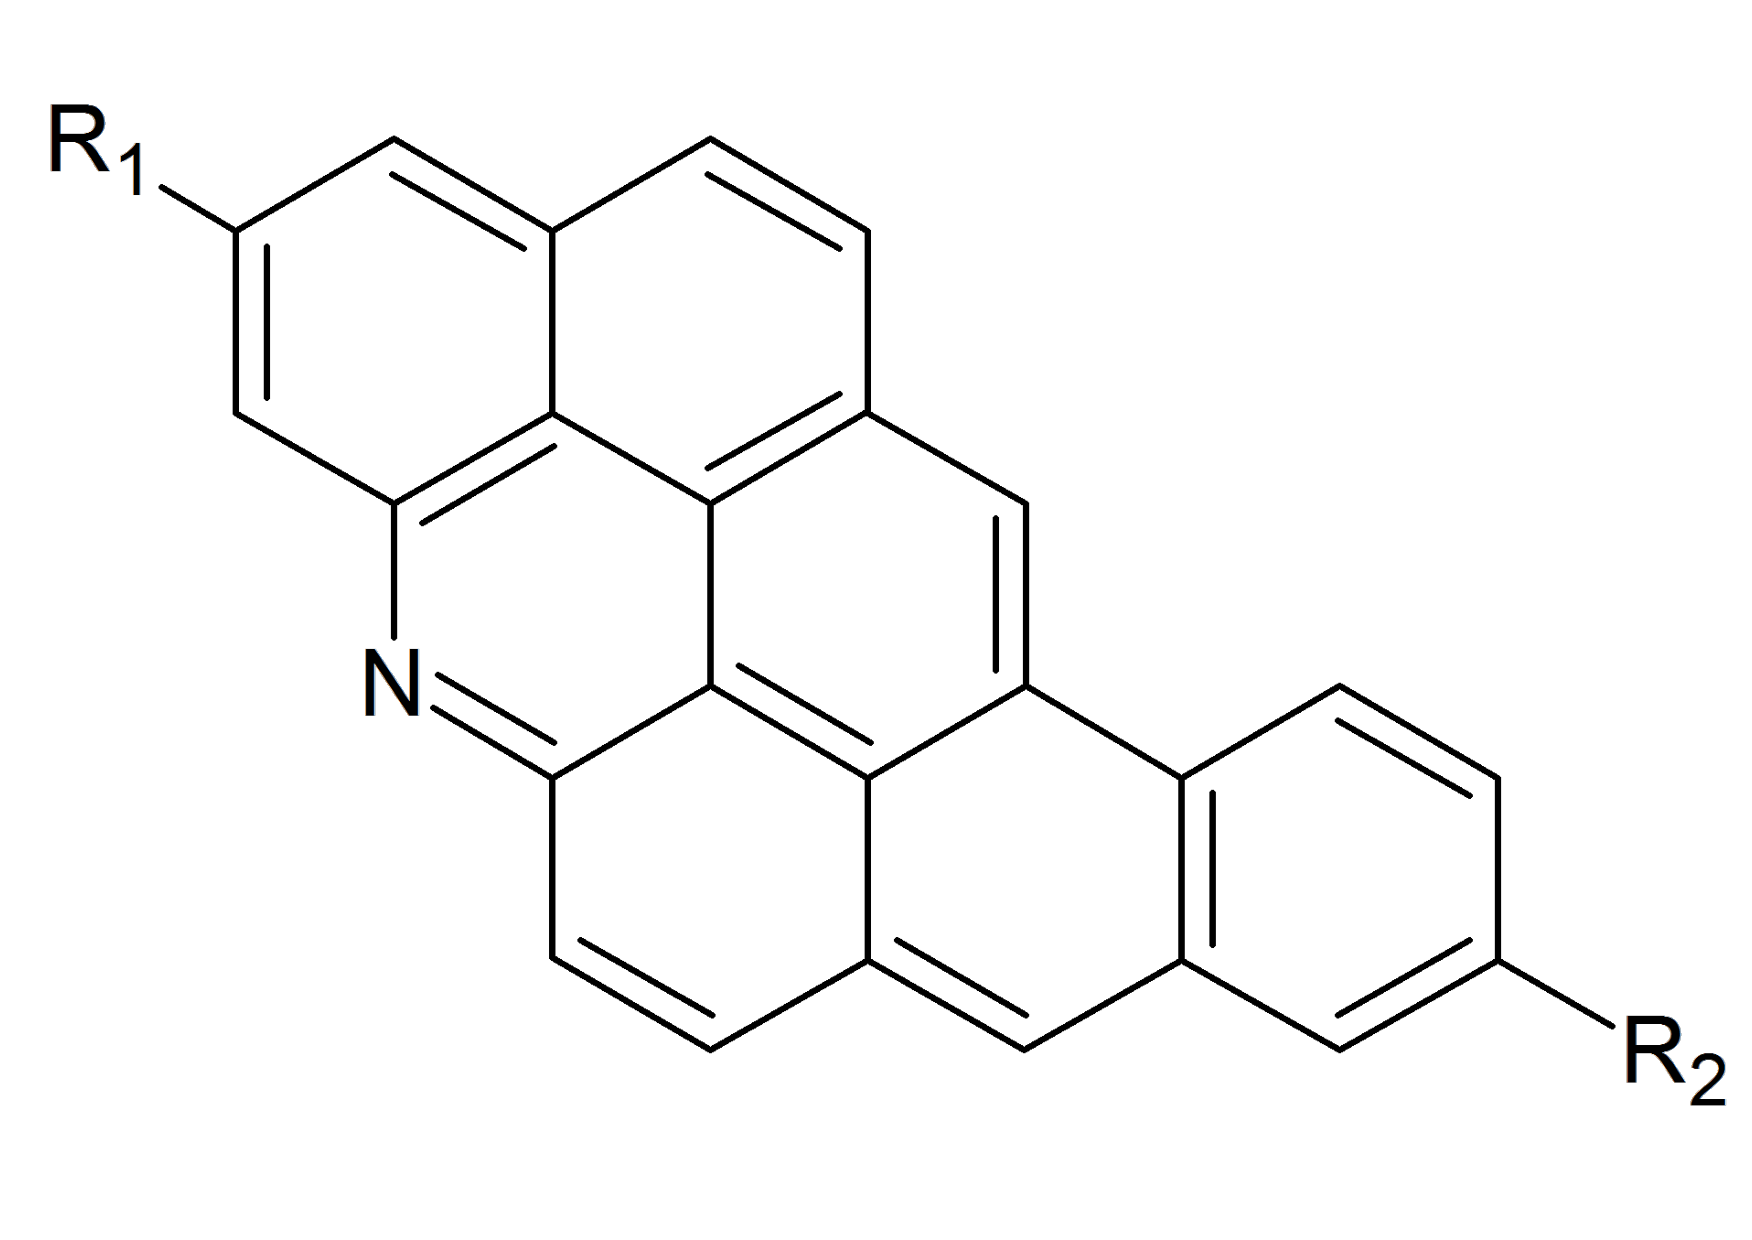
\includegraphics[width=0.35\columnwidth]{image/CA22}\\
		(a) & (b)\\
	\end{tabular}
	\caption{Two different asphaltene structures found in the crude petroleum: (a) PA3 and (b) CA22. $R_1$ and $R_2$ are the $n$-hexyl lateral chains which can have \ce{-COOH} or \ce{-CH3} as chain-ends. $X_n$ (n=1-3) can be \ce{O}, \ce{S}, or \ce{NH} atom groups.}
	\label{pap:fig02}
\end{figure}

These molecules had their lateral chain-end varied as well as the heteroatom on their conjugated cores. This allowed us to have 14 different molecular structures that were studied separately and together in different proportions. In this way, the aim of this paper is to study the first steps of the asphaltene nano-aggregation by molecular dynamics simulations (MD) as a function of their chemical composition. For PA3, the choice of the heteroatom was motivated by previous  Fourier transform ion cyclotron resonance mass spectroscopy (FT-ICR-MS) results indicating their presence in the aromatic core.\cite{kim2009automated,stanford2007compositional} In the case of CA22, nitrogen was chosen because of the relatively high stability of 6-atoms cycle compared to what can be obtained using the other heteroatoms. These molecules were declined following the tabulation in Table \ref{pap:tab01}. They are classified following their number of carbon atoms (NbC), their Double Bond Equivalent (DBE) and the Class to which they belong accordingly to FT-ICR-MS, \cite{kendrick1963mass,hughey2001kendrick,shi2010characterization} which indexes might be of use for further referring.

\begin{table}[htb]
	\caption{Labelling of the systems used in this study, with the chain-ends of the lateral chains. Molecules A11-A53 are of the type PA3 and AAA, AAB and AAC are of the type CA22. NbC is the number of Carbon atoms of the structure, DBE is the Double Bond Equivalent and Class stands for the nomenclature reporting the number of heteroatoms found in the structure by FT-ICR-MS. $M_w$ is the molecular weight of each molecule.}
	\centering    
	\begin{tabular}{c|ccc|cc|ccc|c}
		\hline 		
		\textbf{Label} & $X_1$ & $X_2$ & $X_3$ & $R_1$ & $R_2$ & NbC & DBE & Class & $M_w$ (g.mol$^{-1}$)  \\
		\hline 
		\textbf{A11} & O & O & O & \ce{COOH} & \ce{COOH} & 45 & 27 & \ce{O7} & 690.8\\
		\textbf{A12} & O & O & O & \ce{CH3} & \ce{COOH} & 45 & 26 & \ce{O5} & 660.8\\
		\textbf{A13} & O & O & O & \ce{CH3} & \ce{CH3} & 45 & 25 & \ce{O3} & 630.8\\
		\textbf{A21} & S & S & S & \ce{COOH} & \ce{COOH} & 45 & 27 & \ce{S3O4} & 740.0\\
		\textbf{A23} & S & S & S & \ce{CH3}& \ce{CH3} & 45 & 25 & \ce{S3} & 679.0 \\
		\textbf{A31} & NH & NH & NH & \ce{COOH} & \ce{COOH} & 45 & 27 & \ce{N3O4} & 687.8 \\
		\textbf{A33} & NH & NH & NH & \ce{CH3} & \ce{CH3} & 45 & 25 & \ce{N3} & 627.8\\
		\textbf{A41} & O & O & S & \ce{COOH} & \ce{COOH} & 45 & 27 & \ce{O6S} & 706.8\\
		\textbf{A43} & O & O & S & \ce{CH3} & \ce{CH3} & 45 & 25 & \ce{O2S} & 646.8 \\
		\textbf{A51} & O & S & S & \ce{COOH} & \ce{COOH} & 45 & 27 & \ce{O5S2} & 723.9\\
		\textbf{A53} & O & S & S & \ce{CH3}& \ce{CH3} & 45 & 25 & \ce{OS2}& 662.9 \\
		\hline
		\textbf{AAA} & - & - & - & \ce{COOH} & \ce{COOH} & 37 & 22 & \ce{N1O4} & 555.6\\
		\textbf{AAB} & - & - & - & \ce{COOH} & \ce{CH3} & 37 & 21 & \ce{N1O2}&525.7 \\
		\textbf{AAC} & - & - & - & \ce{CH3} & \ce{CH3} & 37 & 20 & \ce{N1} & 501.7\\
		\hline
	\end{tabular}
	\label{pap:tab01}
\end{table}

The DBE in this table was calculated as:

\begin{equation}
DBE = C - \frac{H}{2} + \frac{N}{2} +1
\end{equation}

Where C, H and N stand respectively for the number of carbon, hydrogen and nitrogen atoms. The labeling system relies on the following logics: the first ``A'' stands for ``asphaltene'', the second character identifies a different family of molecules: numeric for each type of different molecule within the PA3 family and alphabetic for each type of different molecule within CA22 family. The last character identifies the number of acid chain ends: index 1 for two acid chain ends \ce{-COOH}, index 2 for one acid chain \ce{-COOH} end and one \ce{-CH3} and index 3 for two \ce{-CH3} chain ends (no acid).

For this ensemble of molecules, three distinct scenarios were studied:

\begin{enumerate}
	\item homogeneous boxes - boxes where each asphaltene molecule interacts with its equal;
	\item heterogeneous boxes - boxes where asphaltenes of the same class (PA3 or CA22) are studied among them;
	\item  \textit{super}-heteregenous boxes - boxes where at least one asphaltene molecule is of type PA3 and at least one is of type CA22; 
\end{enumerate}

This variation allowed us to span a large variety of mixing scenarios and to separate the different contributions of each physical-chemical factor having a role on the aggregation of asphaltenes. Finally, it is worthy saying that this work is a follow-up of the one recently published by our group,\cite{sodero2016investigation} in which we have studied the influence of the heteroatom position in a model asphaltene molecule.

However, all the studies available in literature very often take into account the presence of only one type of asphaltene at a time. This approach is not completely representative of the real very complex mixture that is the crude oil and the effect of rationally changing the chemical structure on the aggregation behavior of asphaltenes has, up to our knowledge, never been reported. Some authors have indeed studied the presence of different asphaltenes in the same simulation box but their interest was, mainly, the distribution of each type of molecules across the oil-water interface.\cite{frigerio2011multiscale,mikami2013molecular,yang2015asphaltene}

\section{Simulation Method}

The MD simulations were carried out using the GROMACS 5.1.1 software package.\cite{berendsen1995gromacs,hess2008gromacs,van2005gromacs} The GROMOS96 force field\cite{van1998gromos} with the 53a6 parameter set\cite{oostenbrink2004biomolecular} was used in all calculations. This force field has already been tested on poly-aromatic molecules and has shown to be very useful in the dynamics of this type of system.\cite{teklebrhan2014initial,kuznicki2008molecular,kuznicki2009aggregation,teklebrhan2012probing}

Toluene was used as solvent in order to mimic the infinite dissolution effect and to avoid the formation of the aggregates due to polarity difference. The initial coordinates were used as input to the PRODRG 2.5 server\cite{schuettelkopf2004prodrg} to generate the GROMACS molecular topology and structure files. The topology of toluene molecule was generated from phenylalanine amino acid fraction in GROMACS. This method proved to be precise since it yields a calculated toluene density value of 0.88 g.cm$^{-3}$, in good agreement with the 0.86 g/cm$^{-3}$ value extracted from NIST WebBook (National Institute of Standards and Technology).\cite{nist}

The resulting topologies had their atomic charges adjusted in order to better reproduce the ones obtained by molecular quantum- mechanics methods, such as Density Functional Theory (DFT). 

The C5Pe derivatives had all partial charges for the compounds were used in the topologies based on the GROMOS96 force field parameters. For C=S group, the charges were applied as described by Huang and co-workers.\cite{huang2012molecular} For the molecules based on Schuler \textit{et al.}'s work, the Mulliken charges of the heteroatoms and their surroundings were obtained at the B3LYP/def2-SVP level of theory \cite{becke1993density,lee1988development,stephens1994ab,schafer1992fully,weigend2005balanced} using Orca 3.0.3 software\cite{neese2012orca}.\\

The first part of this study was divided into the study of dimers and trimers; separately, at a fixed concentration. For dimers, cubic boxes of 50 x  50 x 50 \AA~ were either filled randomly with the C5Pe-derivative molecules (random configuration) or filled with two molecules having their poly-aromatic cores are anti-parallel to each other and the aggregate is already formed (this is called the``organized'' configuration), as already mentioned. For the latter case, the spacing between the mass centers of two neighboring asphaltene molecules is 0.35 nm in the -stacking direction. Finally, for both cases, the box was randomly filled with toluene molecules. For trimers, so that the concentration could be kept constant, the simulation boxes now had 50 x  75 x 50 \AA~dimensions. The second part of this study, using the molecules reported by Schuler \textit{et al.}, a cubic box of 50 x  50 x 50 \AA~was randomly filled with 5 molecules of asphaltene and the solvent was then randomly added, as well.\\

Once the several distinct configurations of starting geometries were prepared, their energy was minimized by the steepest descent and conjugated gradients methods. Then, the systems were equilibrated in the NPT ensemble at 298 K and 1 bar pressure during 3 ns using the V-rescale thermostat\cite{bussi2007canonical}\footnote{For the systems using the C5Pe derivatives, the Berendsen thermostat was used for convenience reasons and this has no impact on the results of the calculations.} and Berendsen barostat.\cite{berendsen1984molecular} The production phase consisted of 60 ns of dynamics\footnote{150 ns for the C5Pe derivatives systems.} at 298 K  and 1 bar of pressure also under the NPT ensemble but using the Nosé-Hoover thermostat\cite{hoover1985canonical,nose1984molecular} and the Parrinello-Rahman\cite{parrinello1981polymorphic} pressure coupling algorithm. The initial atomic velocities were set using the Maxwell-Boltzmann distribution of the specified temperature. Throughout minimization, stabilization and production phases, a cutoff of 12 \textup{\AA} was used for both Coulomb and Van der Waals interactions. Periodic boundary conditions were thoroughly applied in the three directions. The Verlet integration algorithm\cite{verlet1967computer} has been used with a 2 fs integration step. The electrostatic interactions were computed using the Particle-Mesh Ewald\cite{essmann1995smooth} summation method with a fast Fourier transform grid spacing of 1.6 \textup{\AA}  to account for long-range electrostatic interactions of the system.  All the bond lengths have been constrained using the LINCS algorithm\cite{hess1997lincs} and this is based on the fact that the bond vibration periods are orders of magnitude quicker than the aggregation process. The neighbor list within 12 \textup{\AA} radius was updated every 5 steps.\\

After minimization, equilibration and production phases, each system was analyzed by calculating the radial distribution function (RDF). These functions are calculated considering the distribution of the distances between the center of mass of the selected residues. In our case, the asphaltene residue is consisted of the aromatic core and the lateral chain. In order to exclude the self-interaction (intra-molecular) configuration, the RDFs were calculated within the interval comprised between 2 and 25 \textup{\AA}. Moreover, the geometry of the poly-aromatic cores was also quantified by the cosine of angle between the poly-aromatic planes. 

%%%%%%%%%%%%%%%%%%%%%%%%%%%%%%%%%%%%%%%%%%%%%%
%     À VOIR SI ÇA VAUT LA PEINE D'INCLURE CE MORCEAU CI-DESSOUS      %
%%%%%%%%%%%%%%%%%%%%%%%%%%%%%%%%%%%%%%%%%%%%%%

%It is worth noting that the average molecular weight of the aggregates, considering Table \ref{pap:tab01}, is of the order of 3200 g.mol$^{-1}$, indicating that our aggregated systems are realistic according to previous experimental works reported in literature (considering the molecular weight of individual asphaltenes to be of the order of $\sim$645 g.mol$^{-1}$).\cite{mullins2008contrasting} In addition, the identified molecules (PA3 and CA22) are only two examples from a complex mixture of thousands of different molecules. Larger systems might lead to slightly different results and other petroleum compounds, such as resins, might also have an effect. The work herein presented is a way of rationalizing the beginning of the aggregation process for slightly different chemical structures and does not have the intention to describe the global behavior of petroleum. Larger systems are envisaged and will be reported soon by our group.

%%%%%%%%%%%%%%%%%%%%%%%%%%%%%%%%%%%%%%%%%%%%%%
%%%%%%%%%%%%%%%%%%%%%%%%%%%%%%%%%%%%%%%%%%%%%%
%%%%%%%%%%%%%%%%%%%%%%%%%%%%%%%%%%%%%%%%%%%%%%


\section{Results and Discussion}

The presentation of the results of both works is done separately in the next sections.

\subsection{C5Pe-derivatives systems}

Molecule 1 was already studied by MDS by Teklebrhan and co-workers\cite{teklebrhan2012probing,teklebrhan2014initial} and Gao and co-workers,\cite{gao2014molecular} with results similar to the ones found in this study, \textit{i.e.}, the dimers of these molecules are stable and keep interacting throughout the simulation. 
Figures \ref{pap:fig03}, \ref{pap:fig04}, \ref{pap:fig05} and \ref{pap:fig06} show the initial (0 ns) and the final configurations (150 ns) of all systems for which the ordered or random starting point was used. Visual inspection of the MDS trajectories indicates that all systems keep their aggregated stack in place throughout the simulation, although some of them, such as 3T, has a final configuration where only two of the asphaltene molecules are in an aggregated state whereas the third is not in interaction with the stack. This is not found for the case where the starting configuration is random, as it can be seen in Figure \ref{pap:fig06}. Further details why this happens are given in the next sections. Thus, the behavior of both dimers and trimers are explained in more details in the next sections. 

\begin{figure}[htb]
	\begin{tabular}{cc}
		 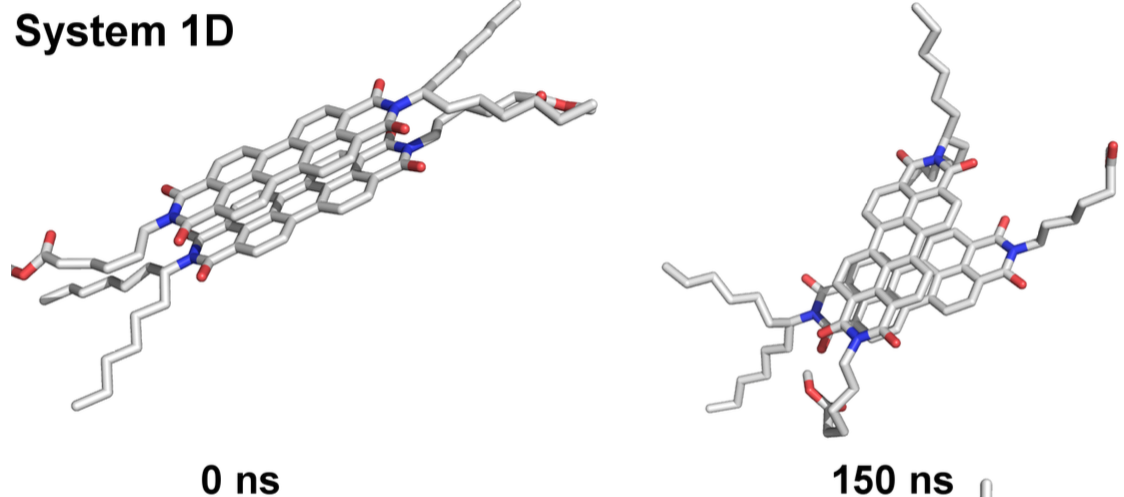
\includegraphics[width=0.45\columnwidth]{image/Figure2a}&
		 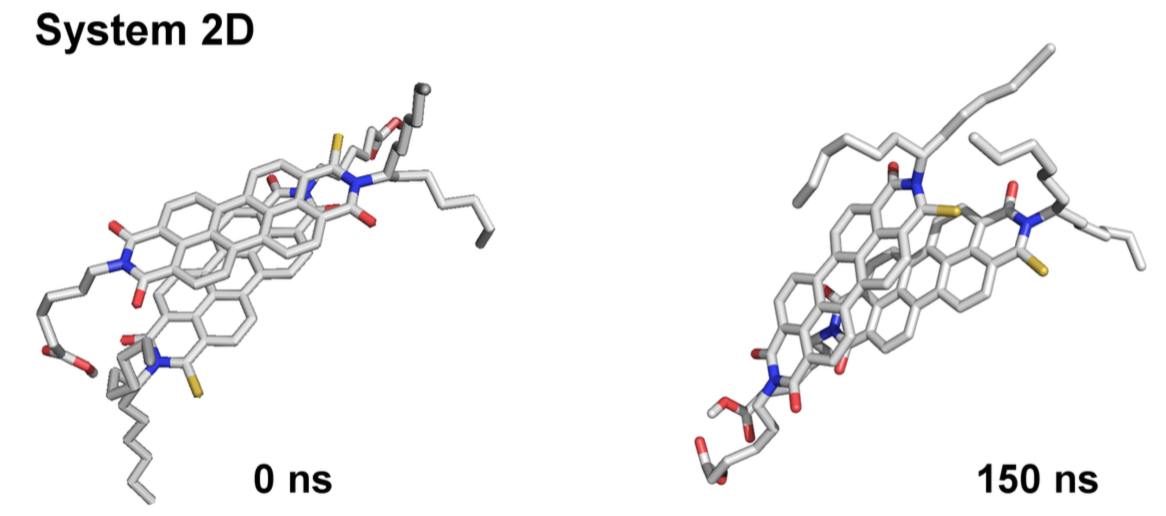
\includegraphics[width=0.45\columnwidth]{image/Figure2b}\\    
		 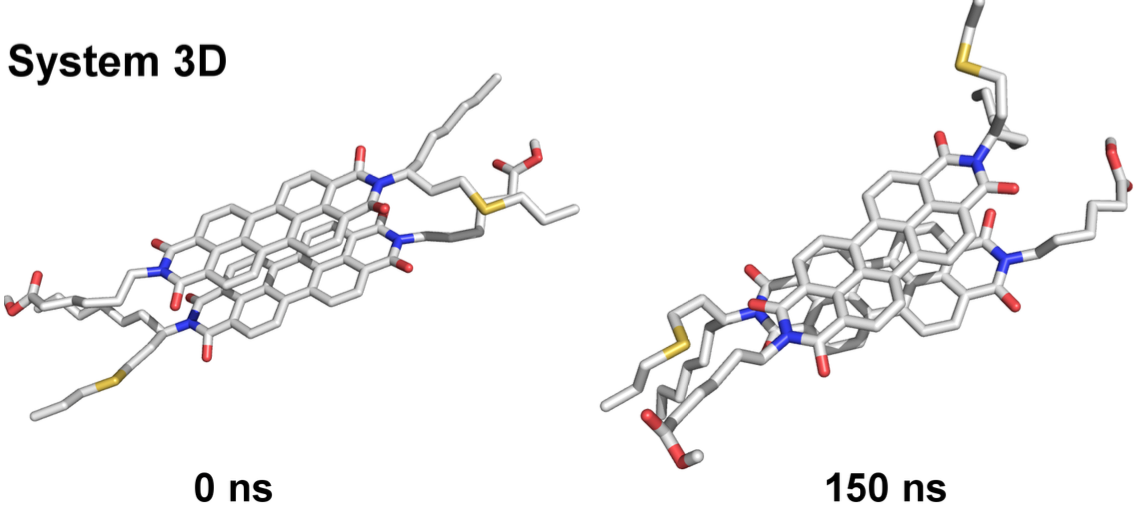
\includegraphics[width=0.45\columnwidth]{image/Figure2c}&     
		 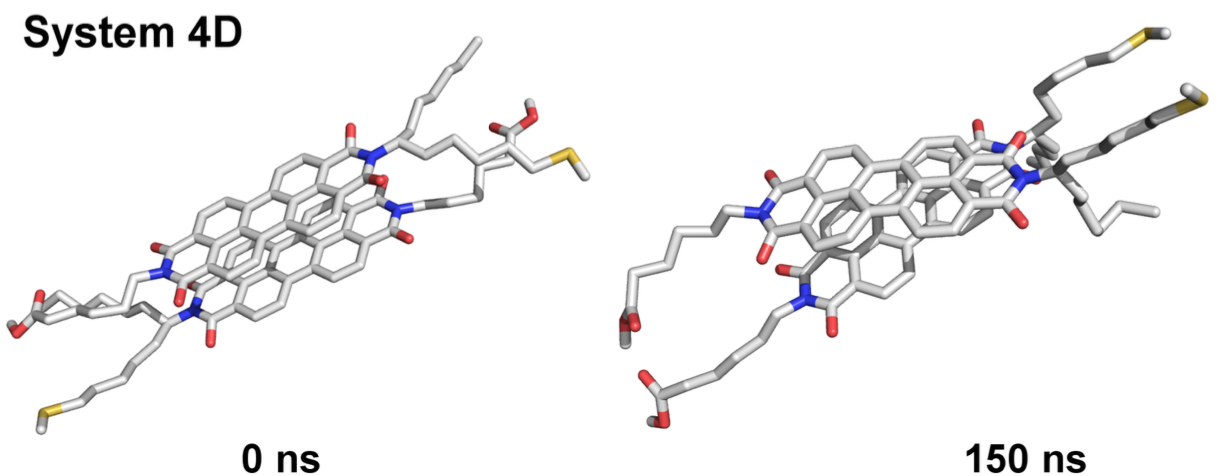
\includegraphics[width=0.45\columnwidth]{image/Figure2d}\\     
		 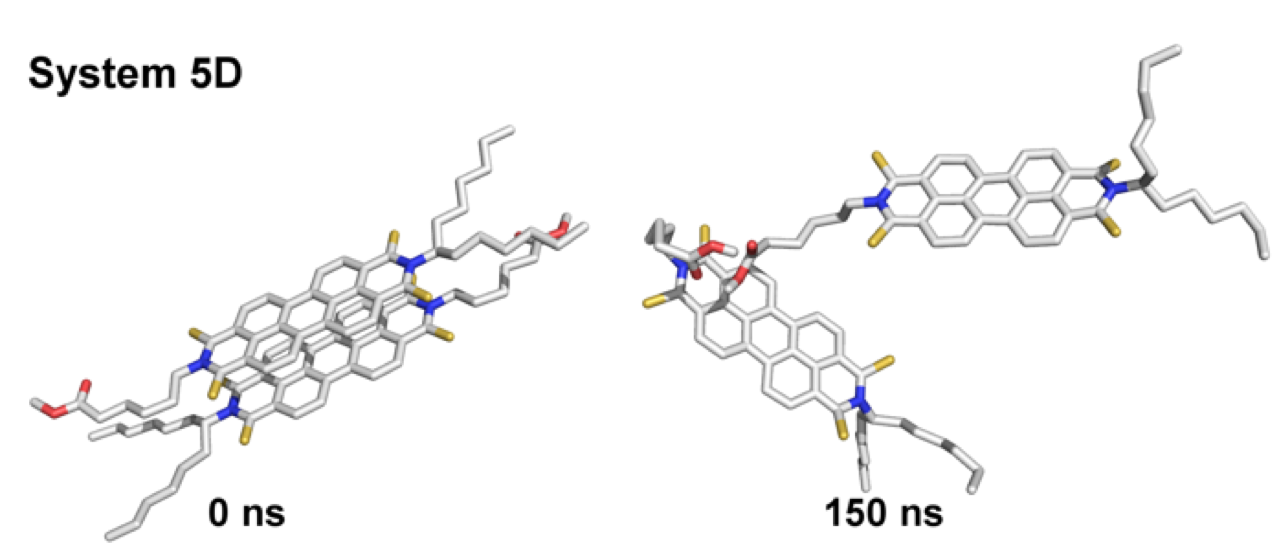
\includegraphics[width=0.45\columnwidth]{image/Figure2e}&
		 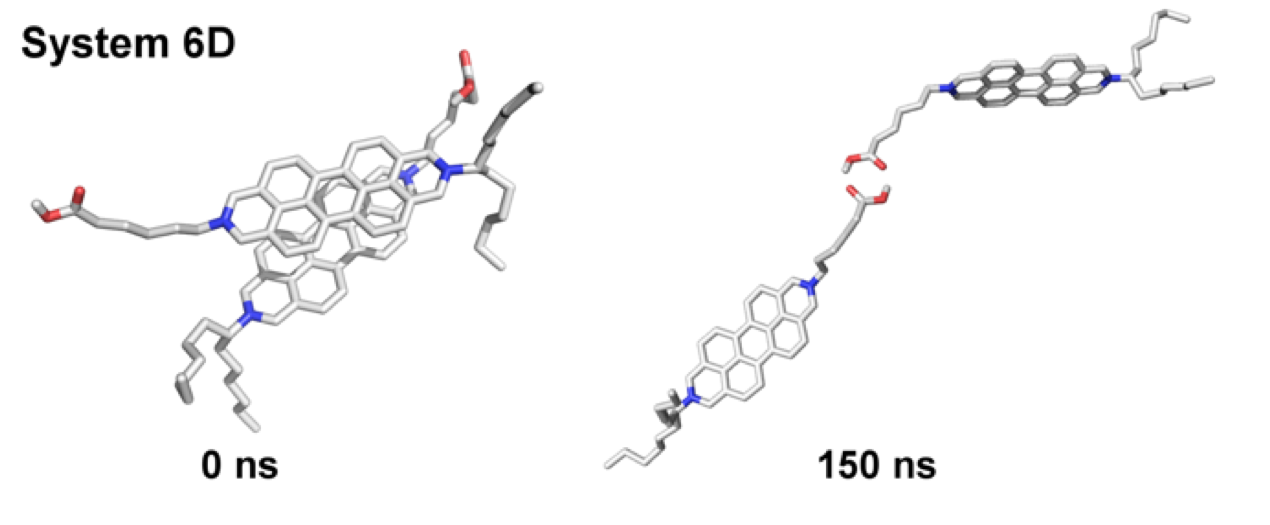
\includegraphics[width=0.45\columnwidth]{image/Figure2f}\\
	\end{tabular}
	\caption{Snapshots of the initial configuration and the final frame of the dimers simulations. Carbon atoms are in grey, oxygen in red, nitrogen in blue and sulfur in yellow. Hydrogen atoms are omitted for clarity.}
	\label{pap:fig03}
\end{figure}

\begin{figure}[htb]
	\begin{tabular}{cccc}
		\small\textbf{System 1D} &  & \small\textbf{System 2D} &\\
		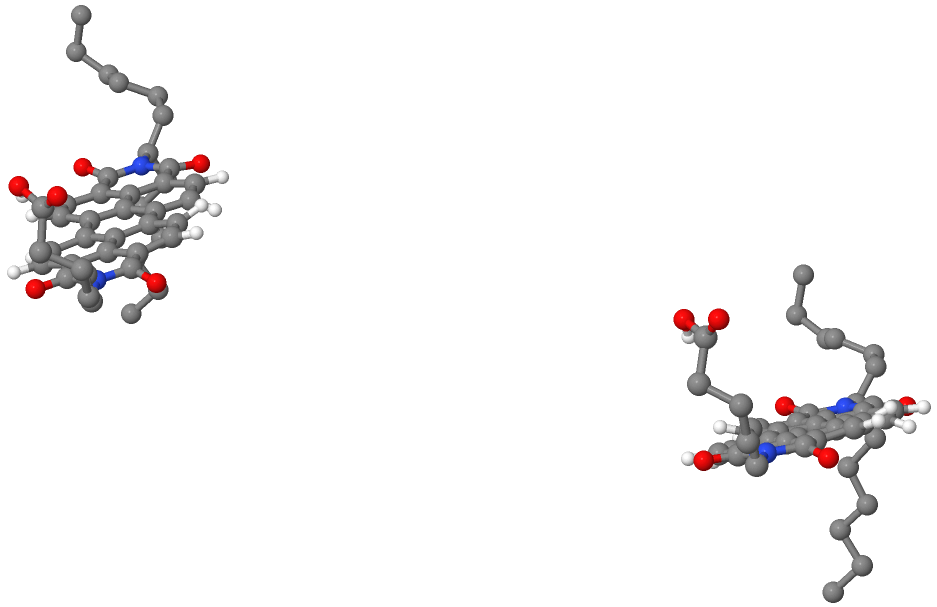
\includegraphics[width=0.2\columnwidth]{image/D_M1_0ns} & 
		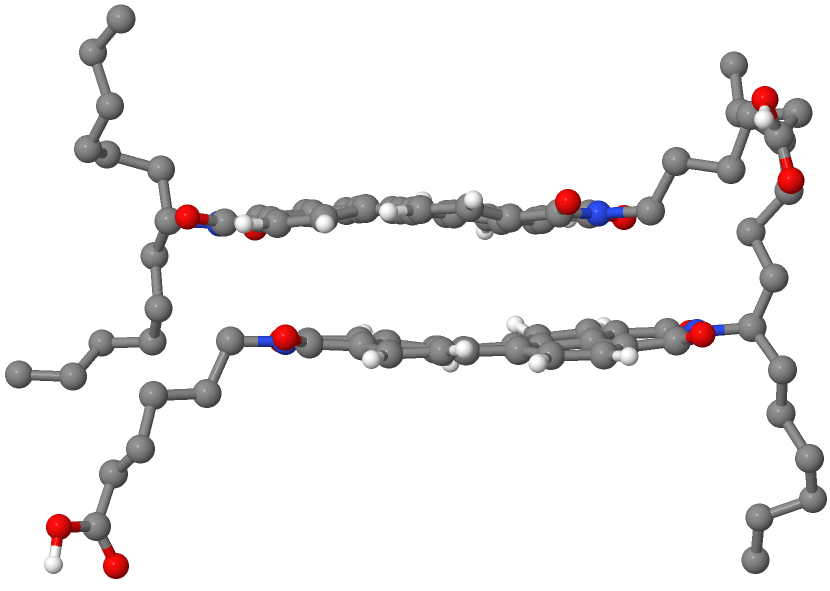
\includegraphics[width=0.2\columnwidth]{image/D_M1_150ns} &
		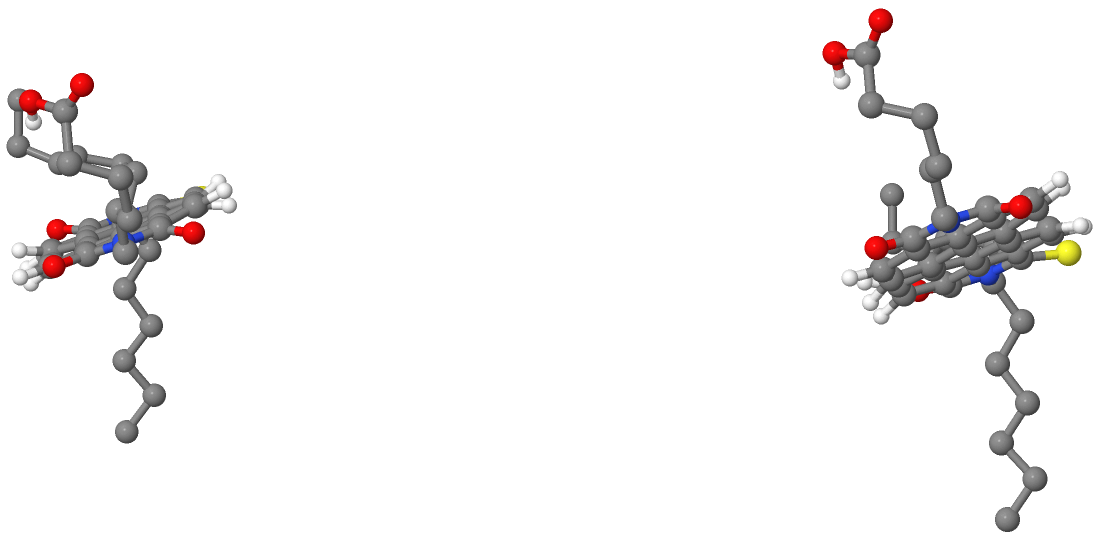
\includegraphics[width=0.2\columnwidth]{image/D_M2_0ns} &
		 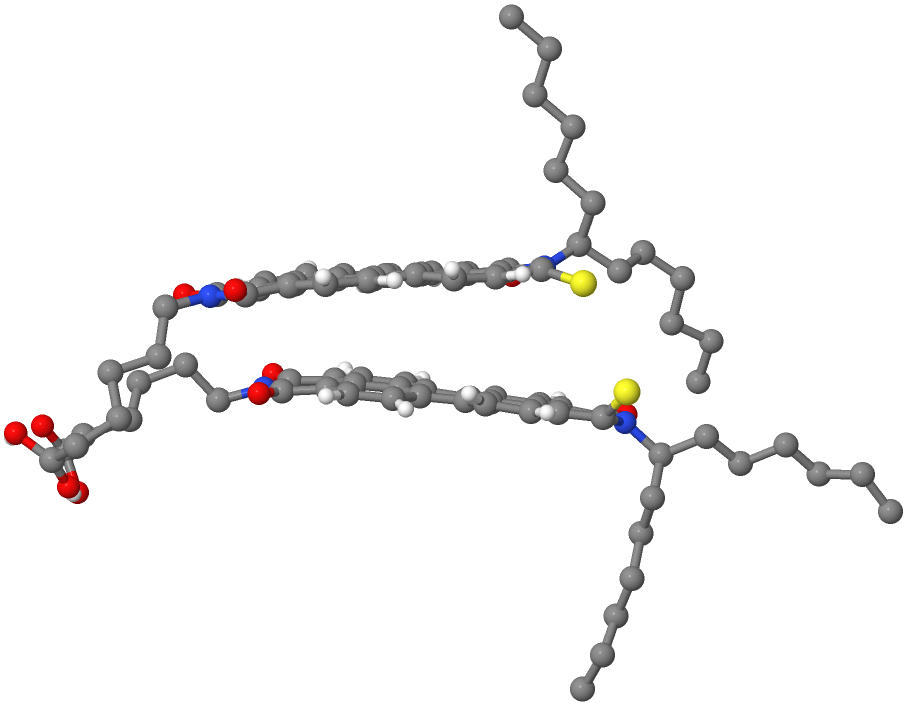
\includegraphics[width=0.2\columnwidth]{image/D_M2_150ns}\\   
		\small\textbf{0 ns} & \small\textbf{150 ns} & \small\textbf{0 ns} & \small\textbf{150 ns} \\
		&&&\\
		\small\textbf{System 3D} &  & \small\textbf{System 4D} &\\
		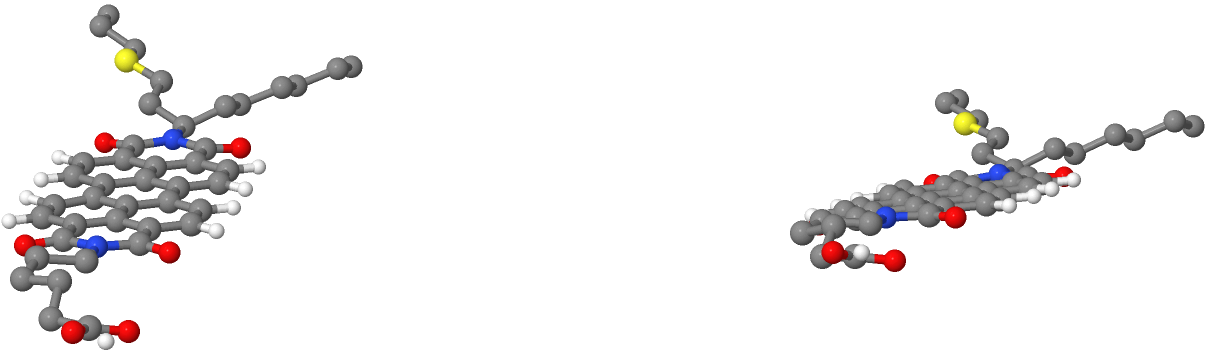
\includegraphics[width=0.2\columnwidth]{image/D_M3_0ns} & 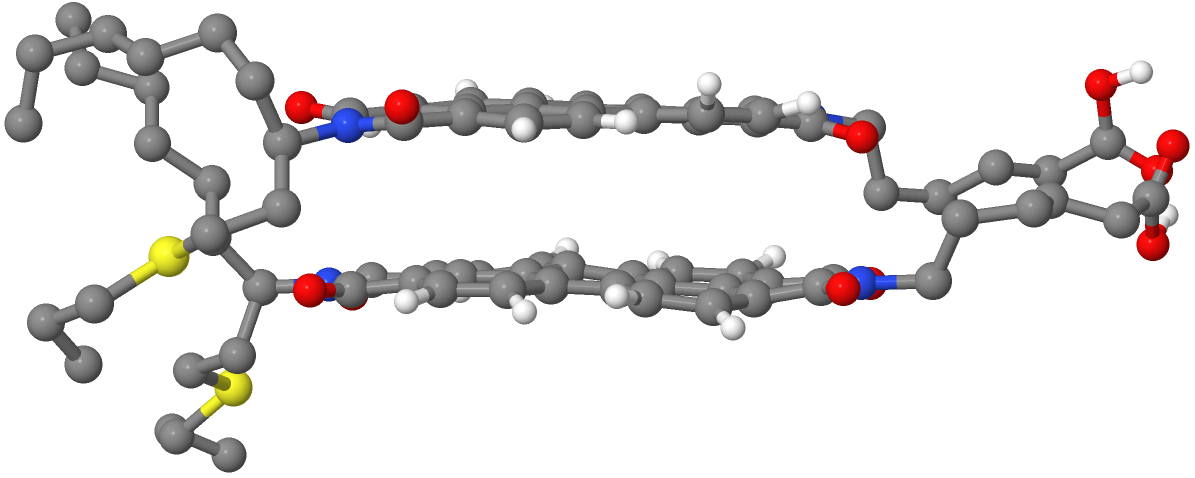
\includegraphics[width=0.2\columnwidth]{image/D_M3_150ns} &
		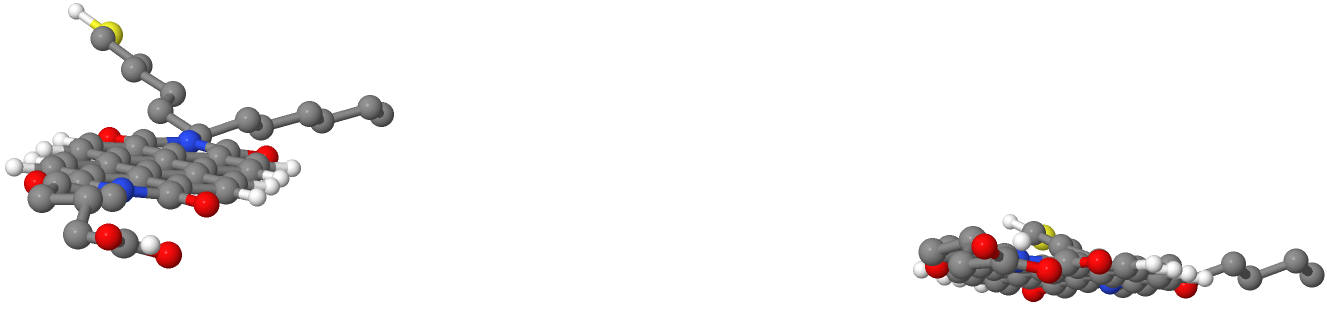
\includegraphics[width=0.2\columnwidth]{image/D_M4_0ns} & 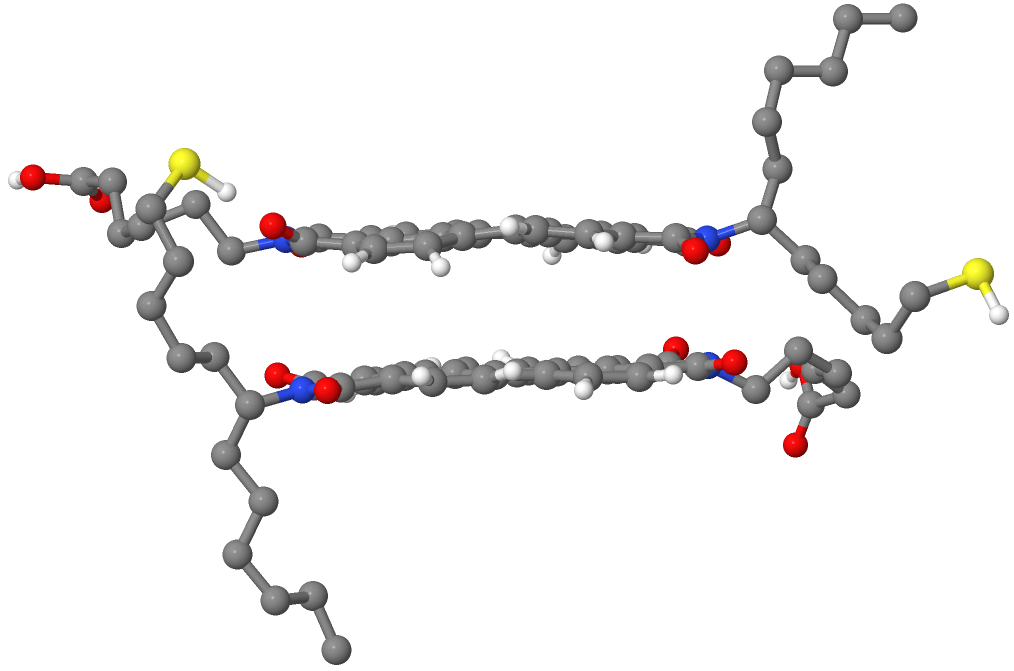
\includegraphics[width=0.2\columnwidth]{image/D_M4_150ns} \\
		\small\textbf{0 ns} & \small\textbf{150 ns} & \small\textbf{0 ns} & \small\textbf{150 ns} \\
		&&&\\
		\small\textbf{System 5D} &  & \small\textbf{System 6D} &\\
		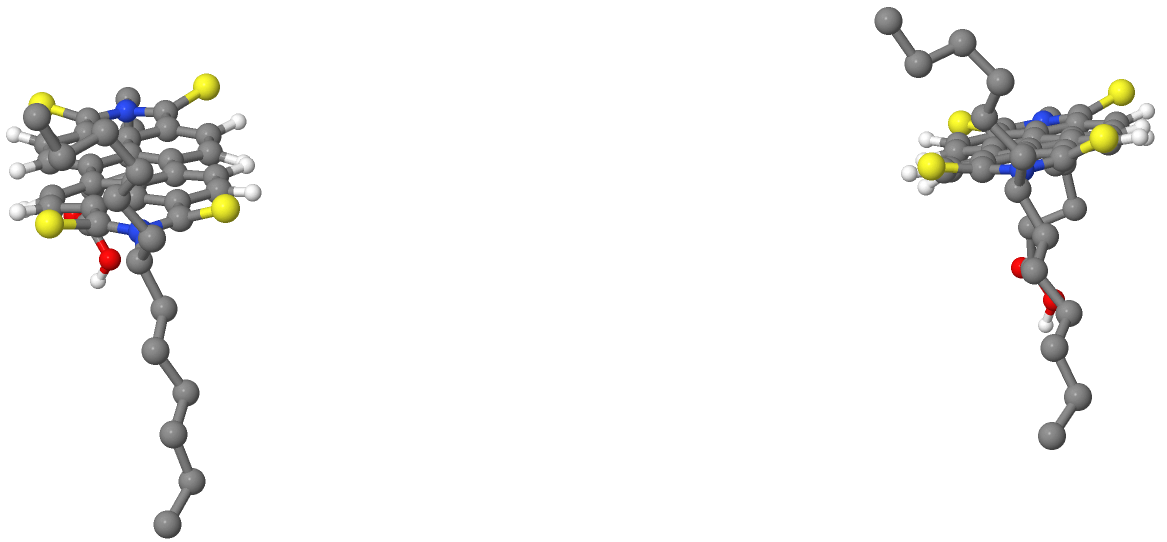
\includegraphics[width=0.2\columnwidth]{image/D_M5_0ns} & 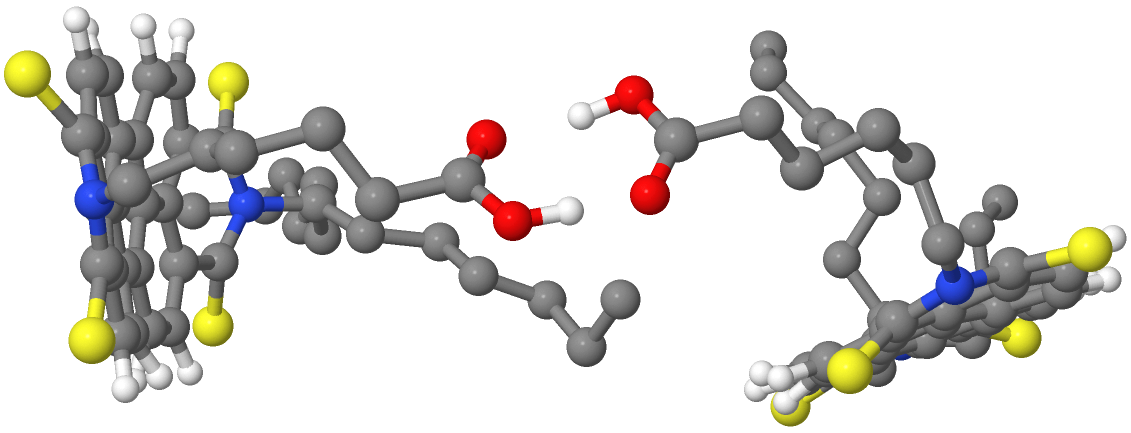
\includegraphics[width=0.2\columnwidth]{image/D_M5_150ns} &
		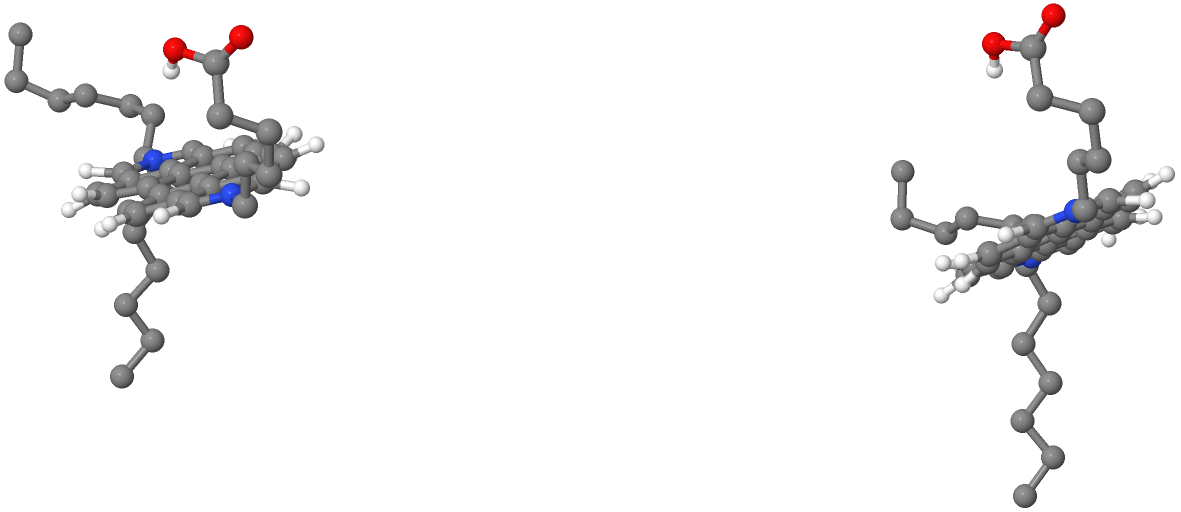
\includegraphics[width=0.2\columnwidth]{image/D_M6_0ns} & 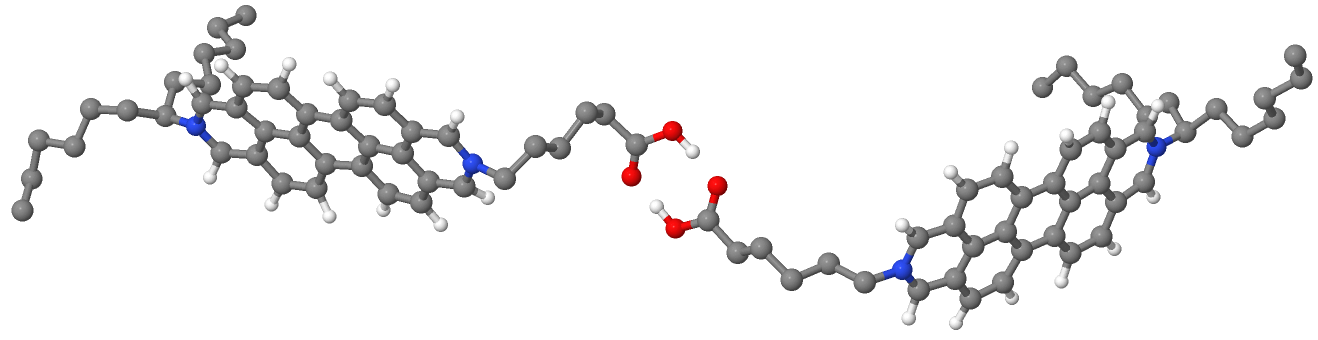
\includegraphics[width=0.2\columnwidth]{image/D_M6_150ns}\\
		\small\textbf{0 ns} & \small\textbf{150 ns} & \small\textbf{0 ns} & \small\textbf{150 ns} \\
	\end{tabular}
	\caption{Snapshots of the initial configuration and the final frame of the dimers simulations for the random disposition case. Carbon atoms are in grey, oxygen in red, nitrogen in blue and sulfur in yellow. Hydrogen atoms are omitted for clarity.}
	\label{pap:fig04}
\end{figure}

\begin{figure}[H]
	\begin{tabular}{cc}
		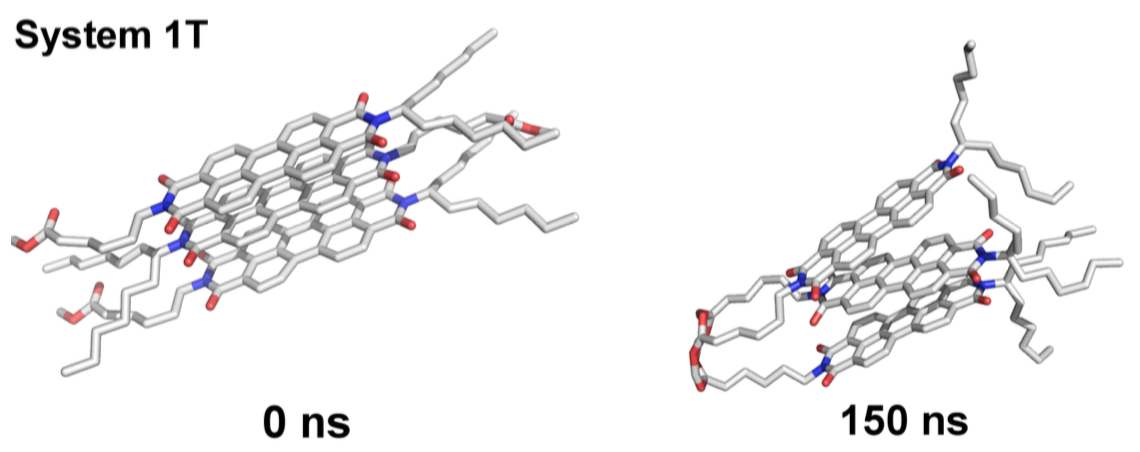
\includegraphics[width=0.45\columnwidth]{image/Figure3a}&
		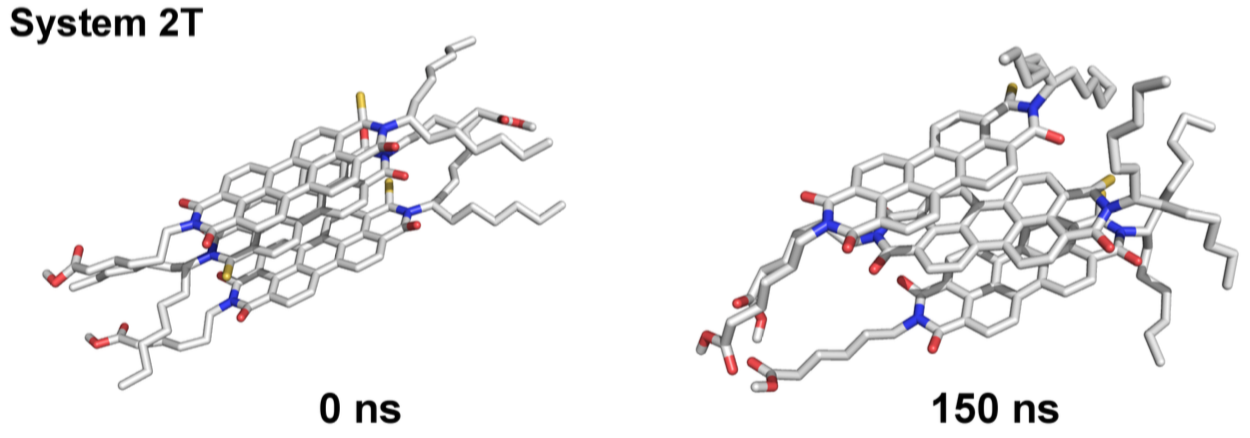
\includegraphics[width=0.45\columnwidth]{image/Figure3b}\\
		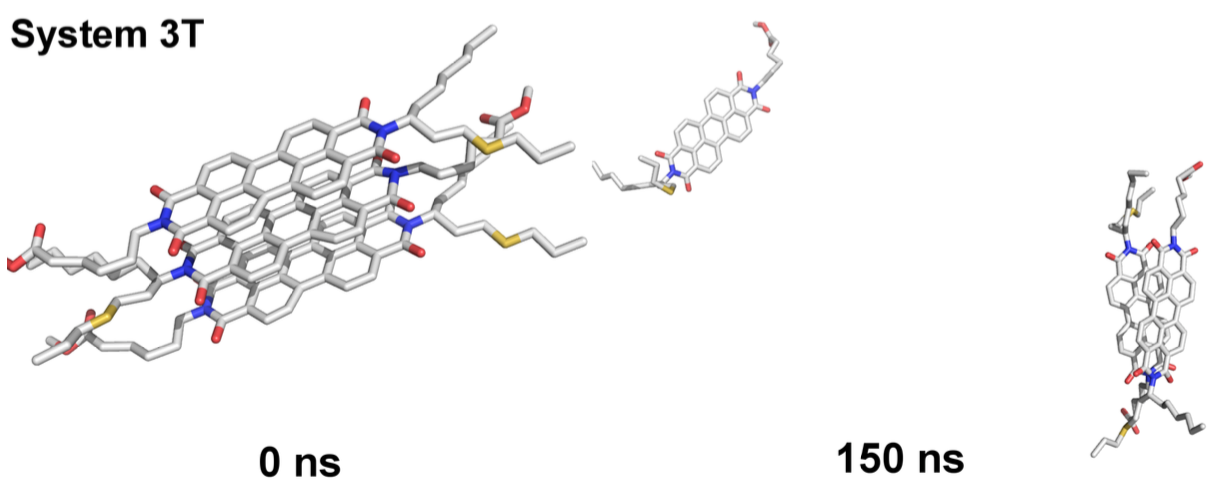
\includegraphics[width=0.45\columnwidth]{image/Figure3c}&
		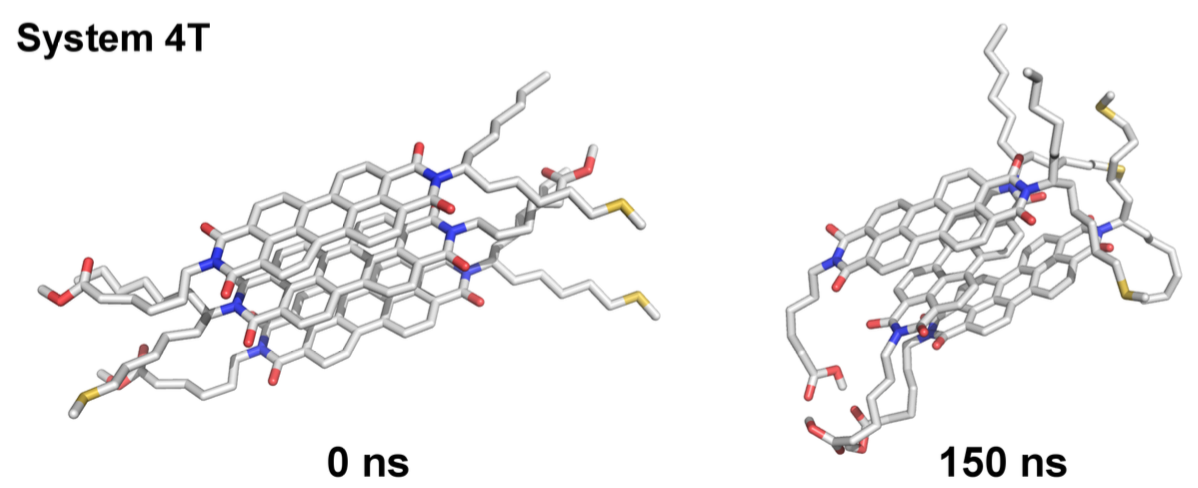
\includegraphics[width=0.45\columnwidth]{image/Figure3d}\\
		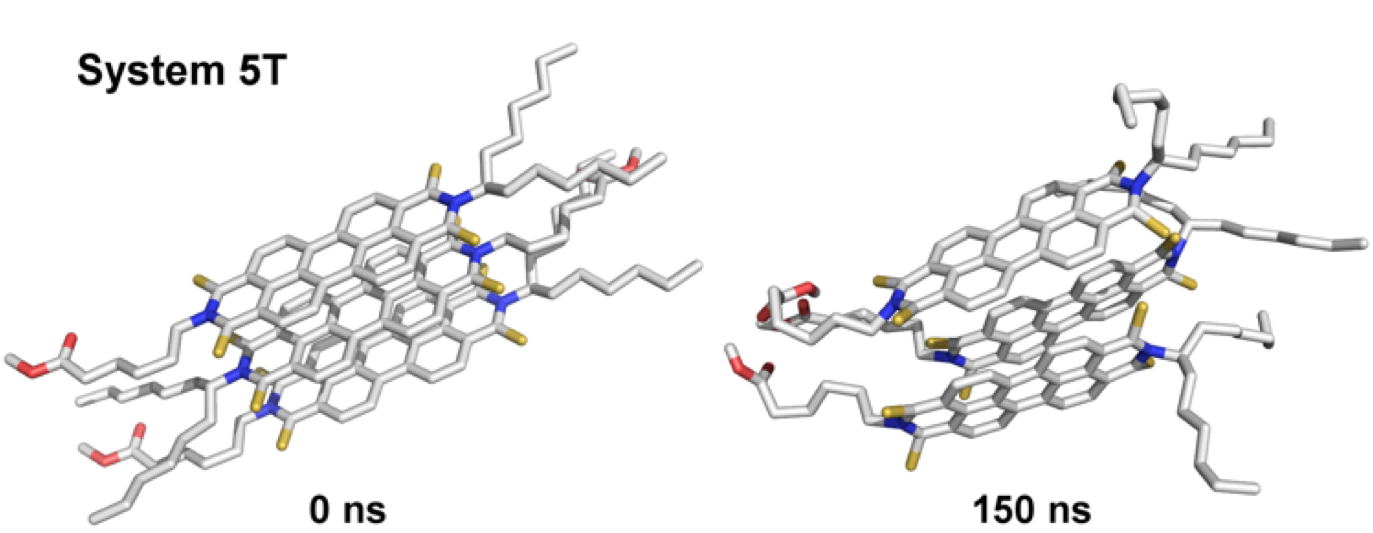
\includegraphics[width=0.45\columnwidth]{image/Figure3e}&
		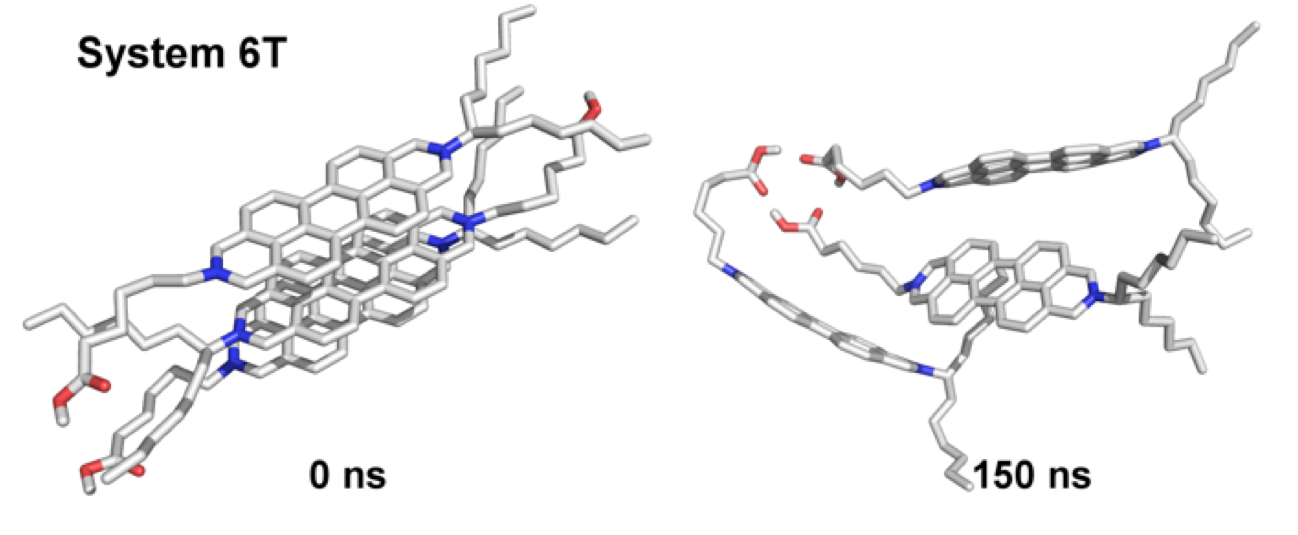
\includegraphics[width=0.45\columnwidth]{image/Figure3f}\\                
	\end{tabular}
	\caption{Snapshots of the initial configuration and the final frame of the trimers simulations. Carbon atoms are in grey, oxygen in red, nitrogen in blue and sulfur in yellow. Hydrogen atoms are omitted for clarity.}
	\label{pap:fig05}
\end{figure}

\begin{figure}[htb]
	\begin{tabular}{cccc}
		\small\textbf{System 1T} &  & \small\textbf{System 2T} &\\
		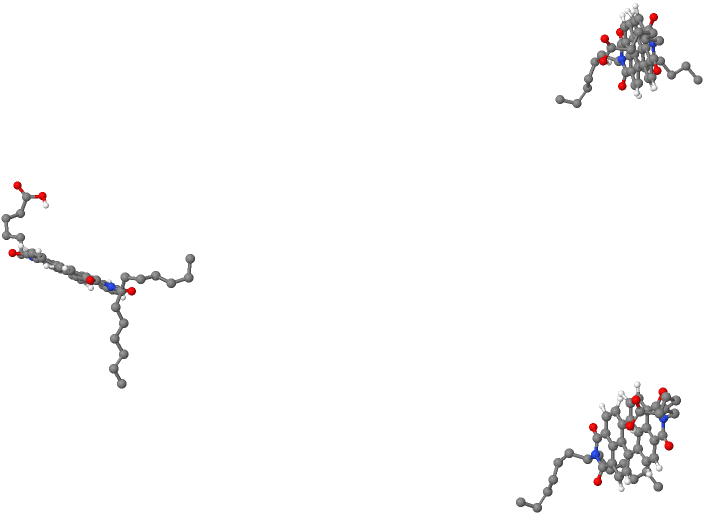
\includegraphics[width=0.2\columnwidth]{image/T_M1_0ns} & 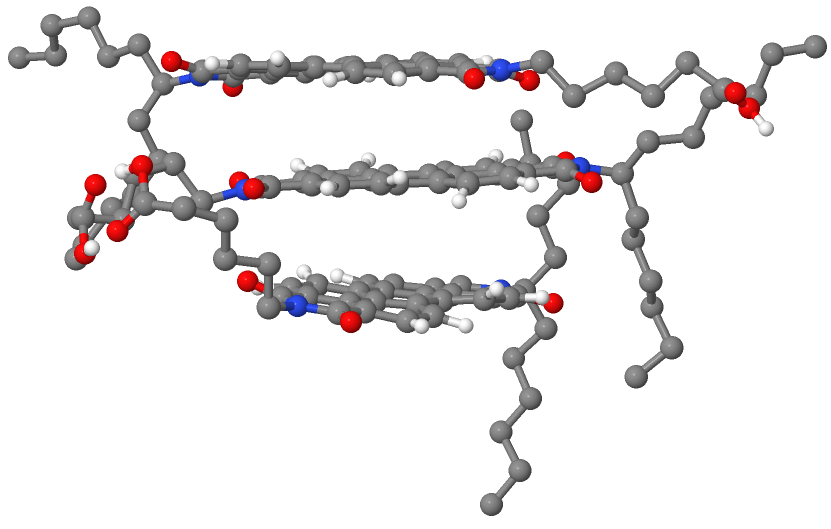
\includegraphics[width=0.2\columnwidth]{image/T_M1_150ns} &
		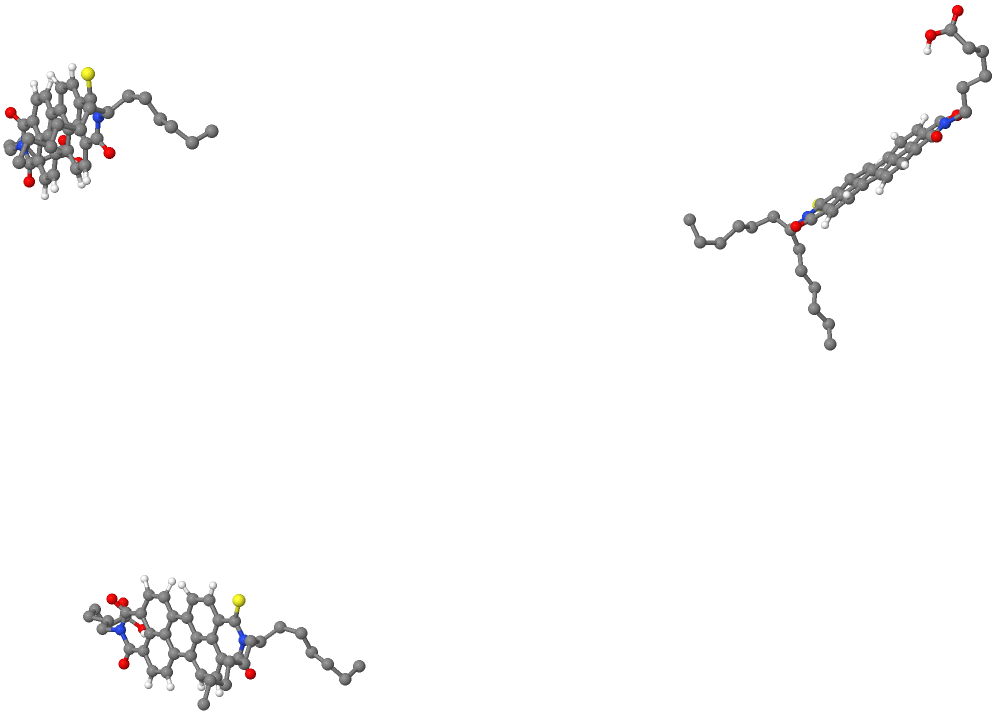
\includegraphics[width=0.2\columnwidth]{image/T_M2_0ns} & 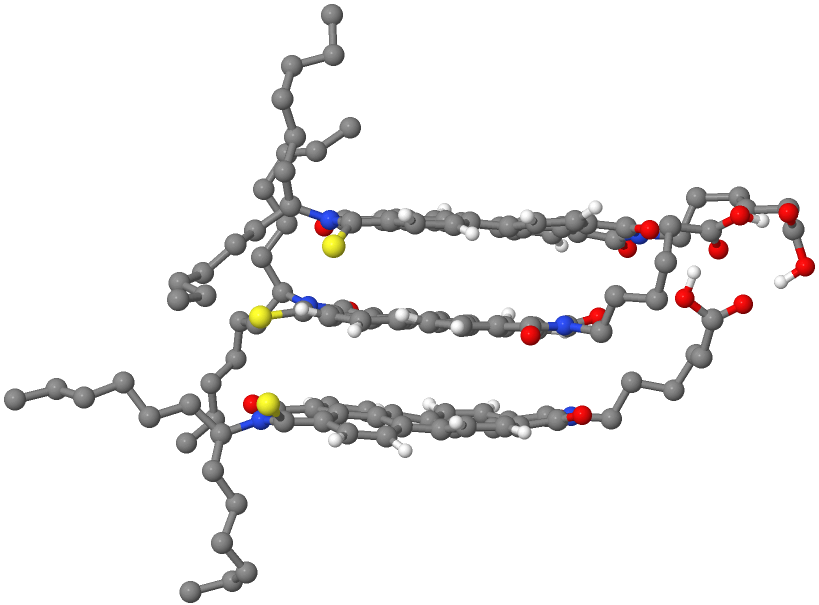
\includegraphics[width=0.2\columnwidth]{image/T_M2_150ns} \\   
		\small\textbf{0 ns} & \small\textbf{150 ns} & \small\textbf{0 ns} & \small\textbf{150 ns} \\
		&&&\\
		\small\textbf{System 3T} &  & \small\textbf{System 4T} &\\
		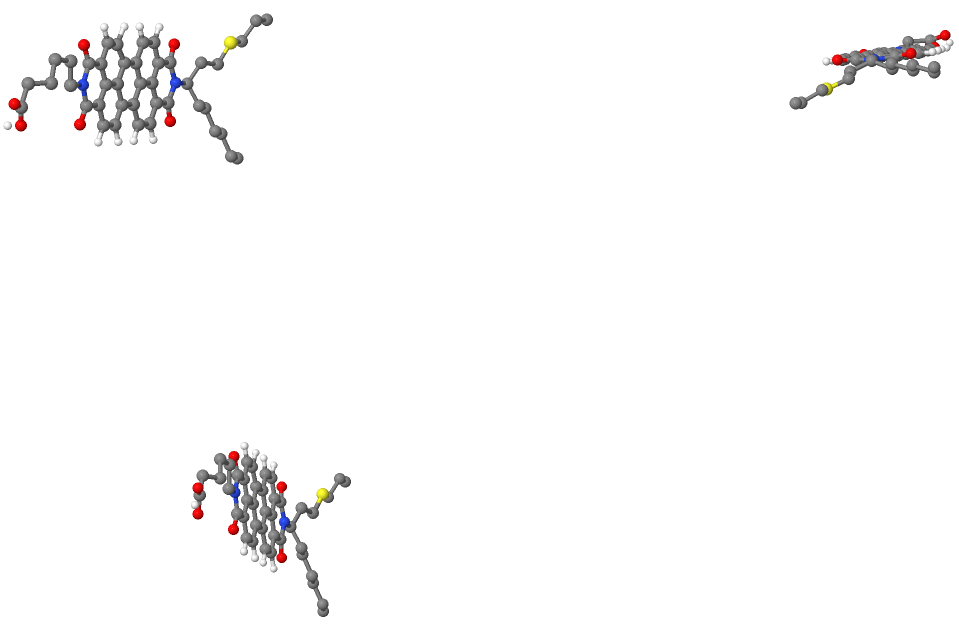
\includegraphics[width=0.2\columnwidth]{image/T_M3_0ns} & 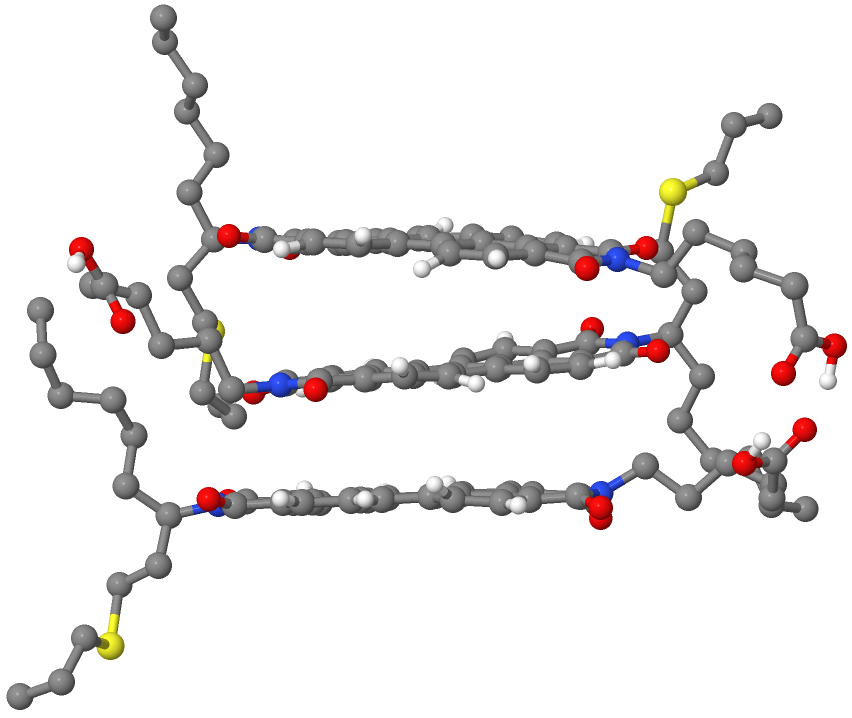
\includegraphics[width=0.2\columnwidth]{image/T_M3_150ns} &
		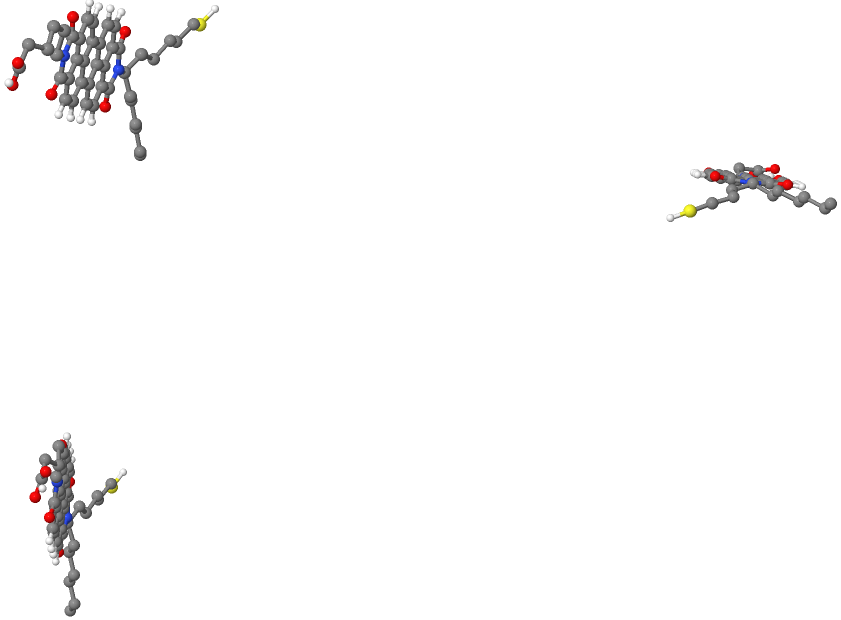
\includegraphics[width=0.2\columnwidth]{image/T_M4_0ns} & 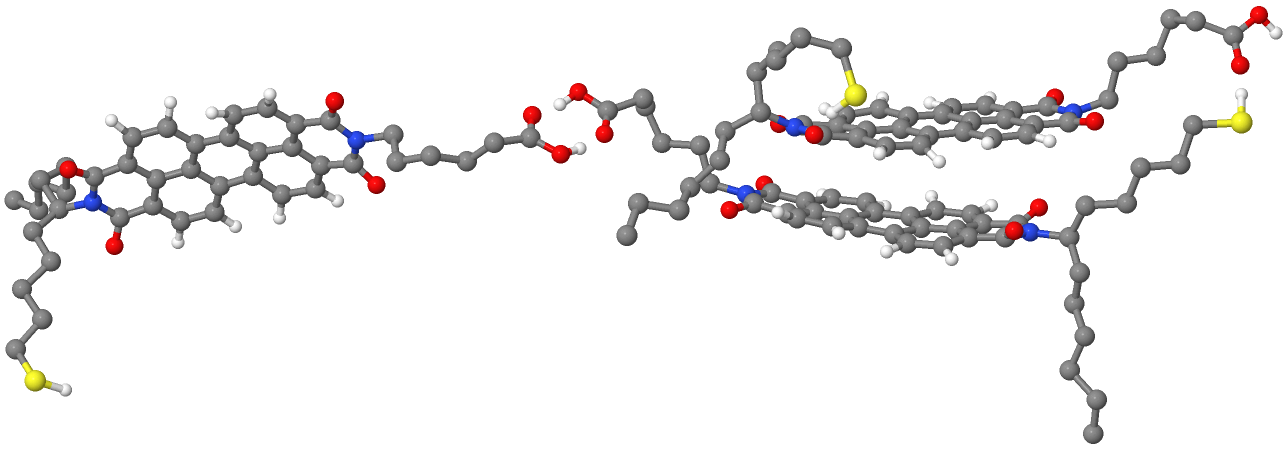
\includegraphics[width=0.2\columnwidth]{image/T_M4_150ns} \\
		\small\textbf{0 ns} & \small\textbf{150 ns} & \small\textbf{0 ns} & \small\textbf{150 ns} \\
		&&&\\
		\small\textbf{System 5T} &  & \small\textbf{System 6T} &\\
		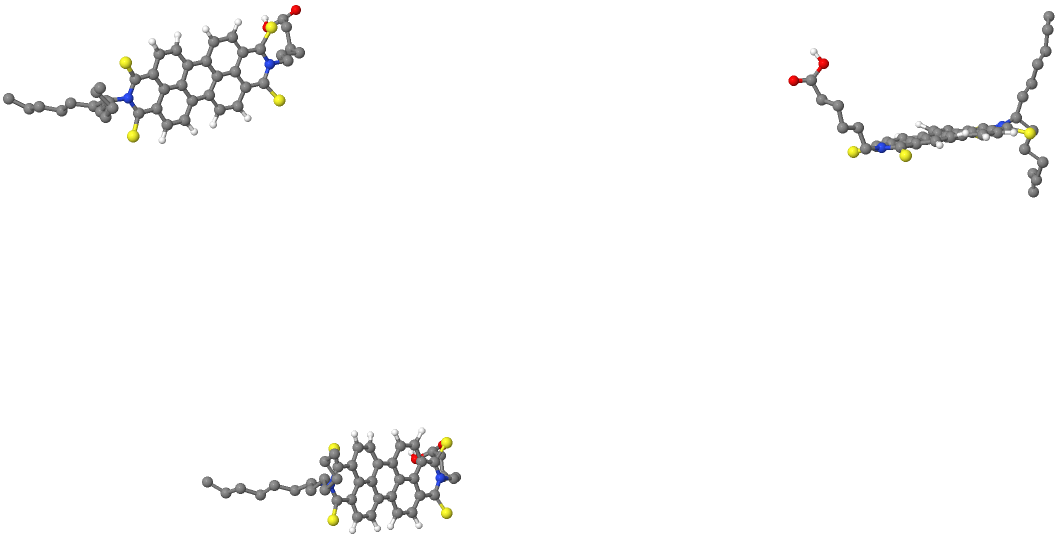
\includegraphics[width=0.2\columnwidth]{image/T_M5_0ns} & 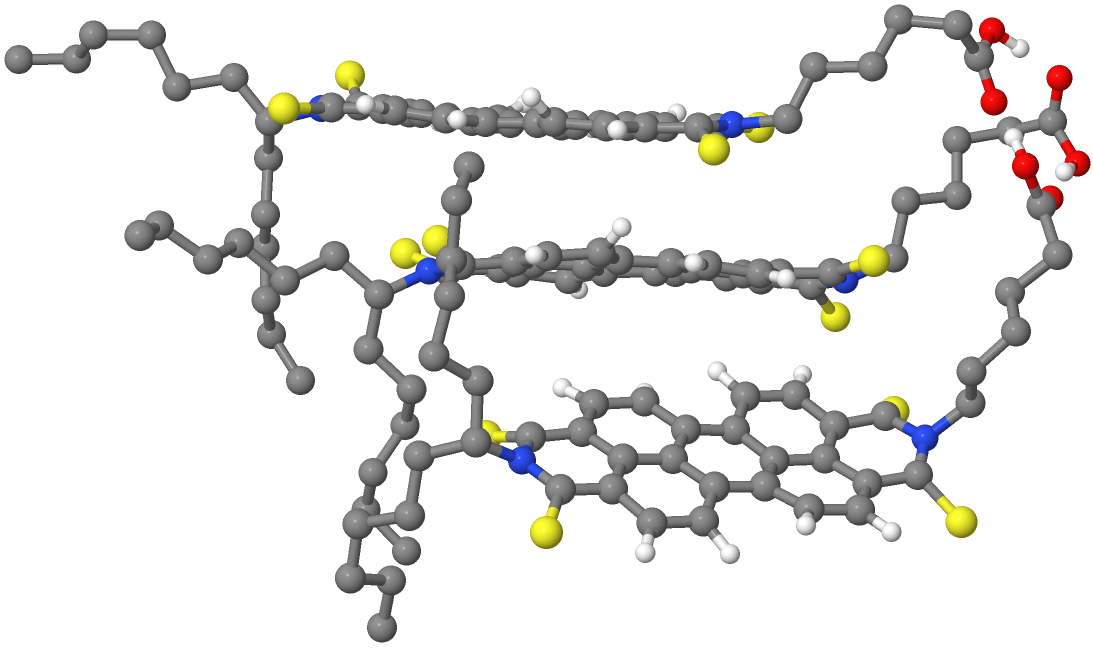
\includegraphics[width=0.2\columnwidth]{image/T_M5_150ns} &
		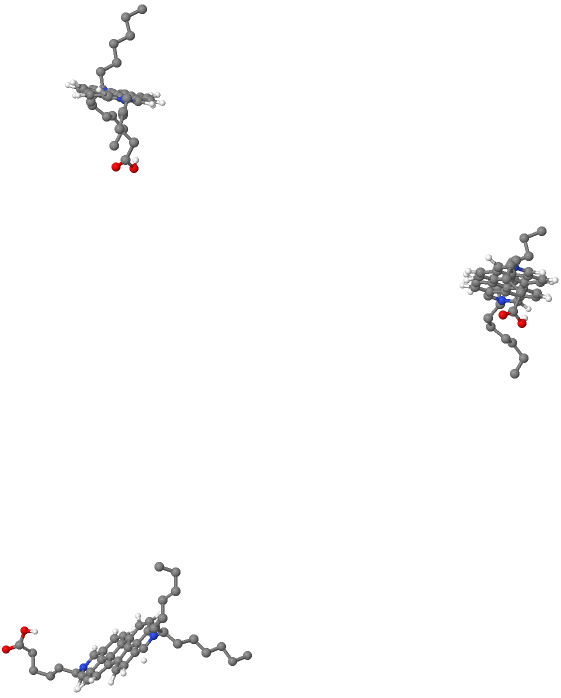
\includegraphics[width=0.2\columnwidth]{image/T_M6_0ns} & 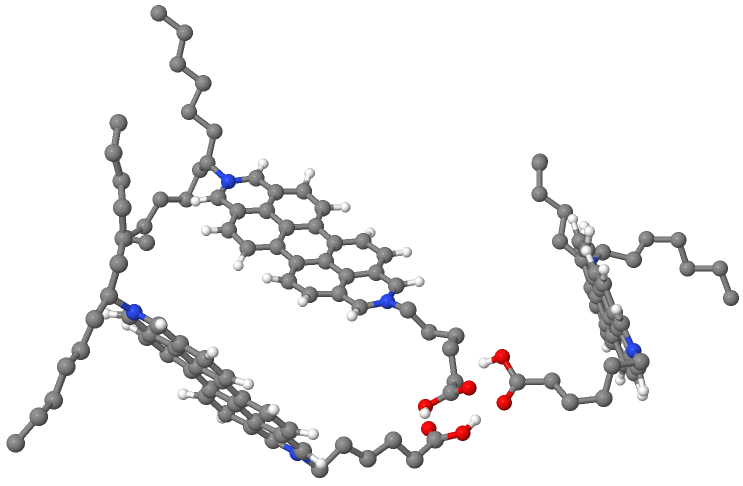
\includegraphics[width=0.2\columnwidth]{image/T_M6_150ns}\\
		\small\textbf{0 ns} & \small\textbf{150 ns} & \small\textbf{0 ns} & \small\textbf{150 ns} \\
	\end{tabular}
	\caption{Snapshots of the initial configuration and the final frame of the trimers simulations for the random disposition case. Carbon atoms are in grey, oxygen in red, nitrogen in blue and sulfur in yellow. Hydrogen atoms are omitted for clarity.}
	\label{pap:fig06}
\end{figure}

\textbf{Dimers (Systems 1D - 6D)}: The analysis of monomer distances shows that systems 1D through 4D are stable as dimers, regardless the initial configuration within the box (Figure \ref{pap:fig07} and \ref{pap:fig08}). For 1D, the average distance between the two molecules is lower that 0.4 nm during $\sim$ 88\% of the simulation, when the aggregated starting point is used and during 90\% for the random starting point situation. The other systems (2D, 3D and 4D) are also stable and are found in the aggregated state during 85 (96), 94 (98) and 96 (94)\% of the simulation for the ``organized'' (random) starting point. Visual inspection of molecular dynamics simulation (MDS) trajectories indicates that systems 5D and 6D are not stable during the molecular dynamics simulation in toluene and this regardless of the starting configuration. However, the systems presented different behavior. 

For the ``organized'' starting configuration: the monomer from system 5D rotates at the beginning of simulation ($\sim$ 1ns) and becomes separated during the MDS. At system 5T, one monomer rotates at 50 ns followed by side chains interaction. However, this configuration is not stable, since the monomers dissociated after 90 ns. Systems 6D and 6T assume many orientations and remains aggregated during all simulation. Nevertheless, they do not adopt defined geometries. This behavior is typical of an interaction done exclusively by means of the acid chain end via hydrogen bonding. System 5D shows variable distances after 30 ns (Figure \ref{pap:fig07}). The molecules are close to each other (< 0.4 nm) at only 15.4\% (23 ns) of the simulation. System 6D shows instability since the beginning of simulation, with distances higher than 0.4 nm during the simulation time.  

\begin{figure}[htb]
	\centering
	\begin{tabular}{cc}
		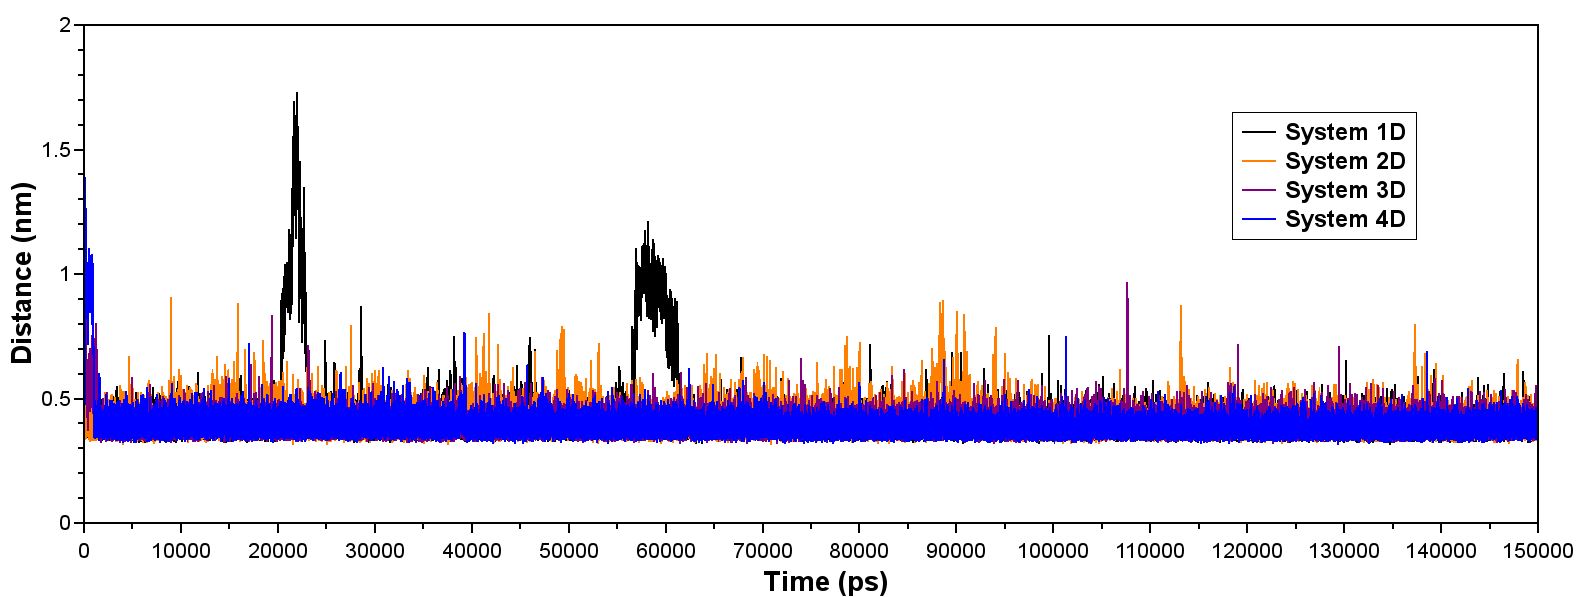
\includegraphics[width=0.45\columnwidth]{image/Figure4}&
		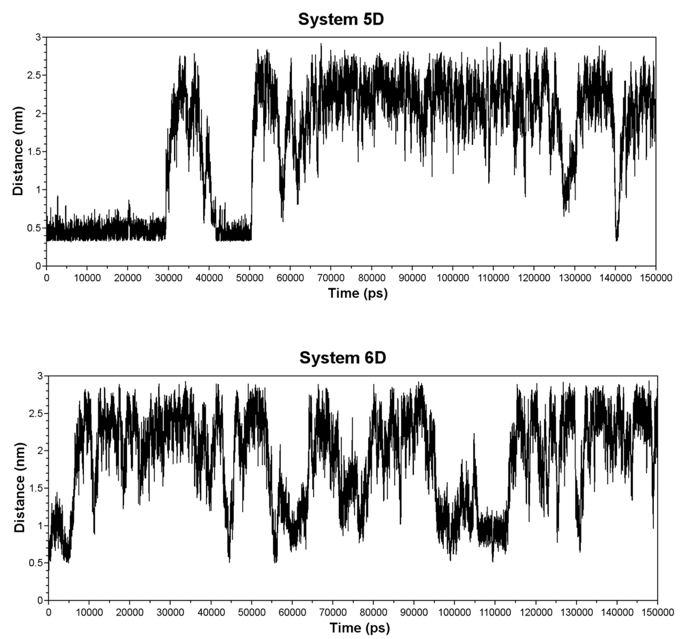
\includegraphics[width=0.45\columnwidth]{image/Figure4b}\\
	\end{tabular}
	\caption{Distances between monomers for ``organized'' starting point.}
	\label{pap:fig07}
\end{figure}

\begin{figure}[htb]
	\centering
	\begin{tabular}{cc}
		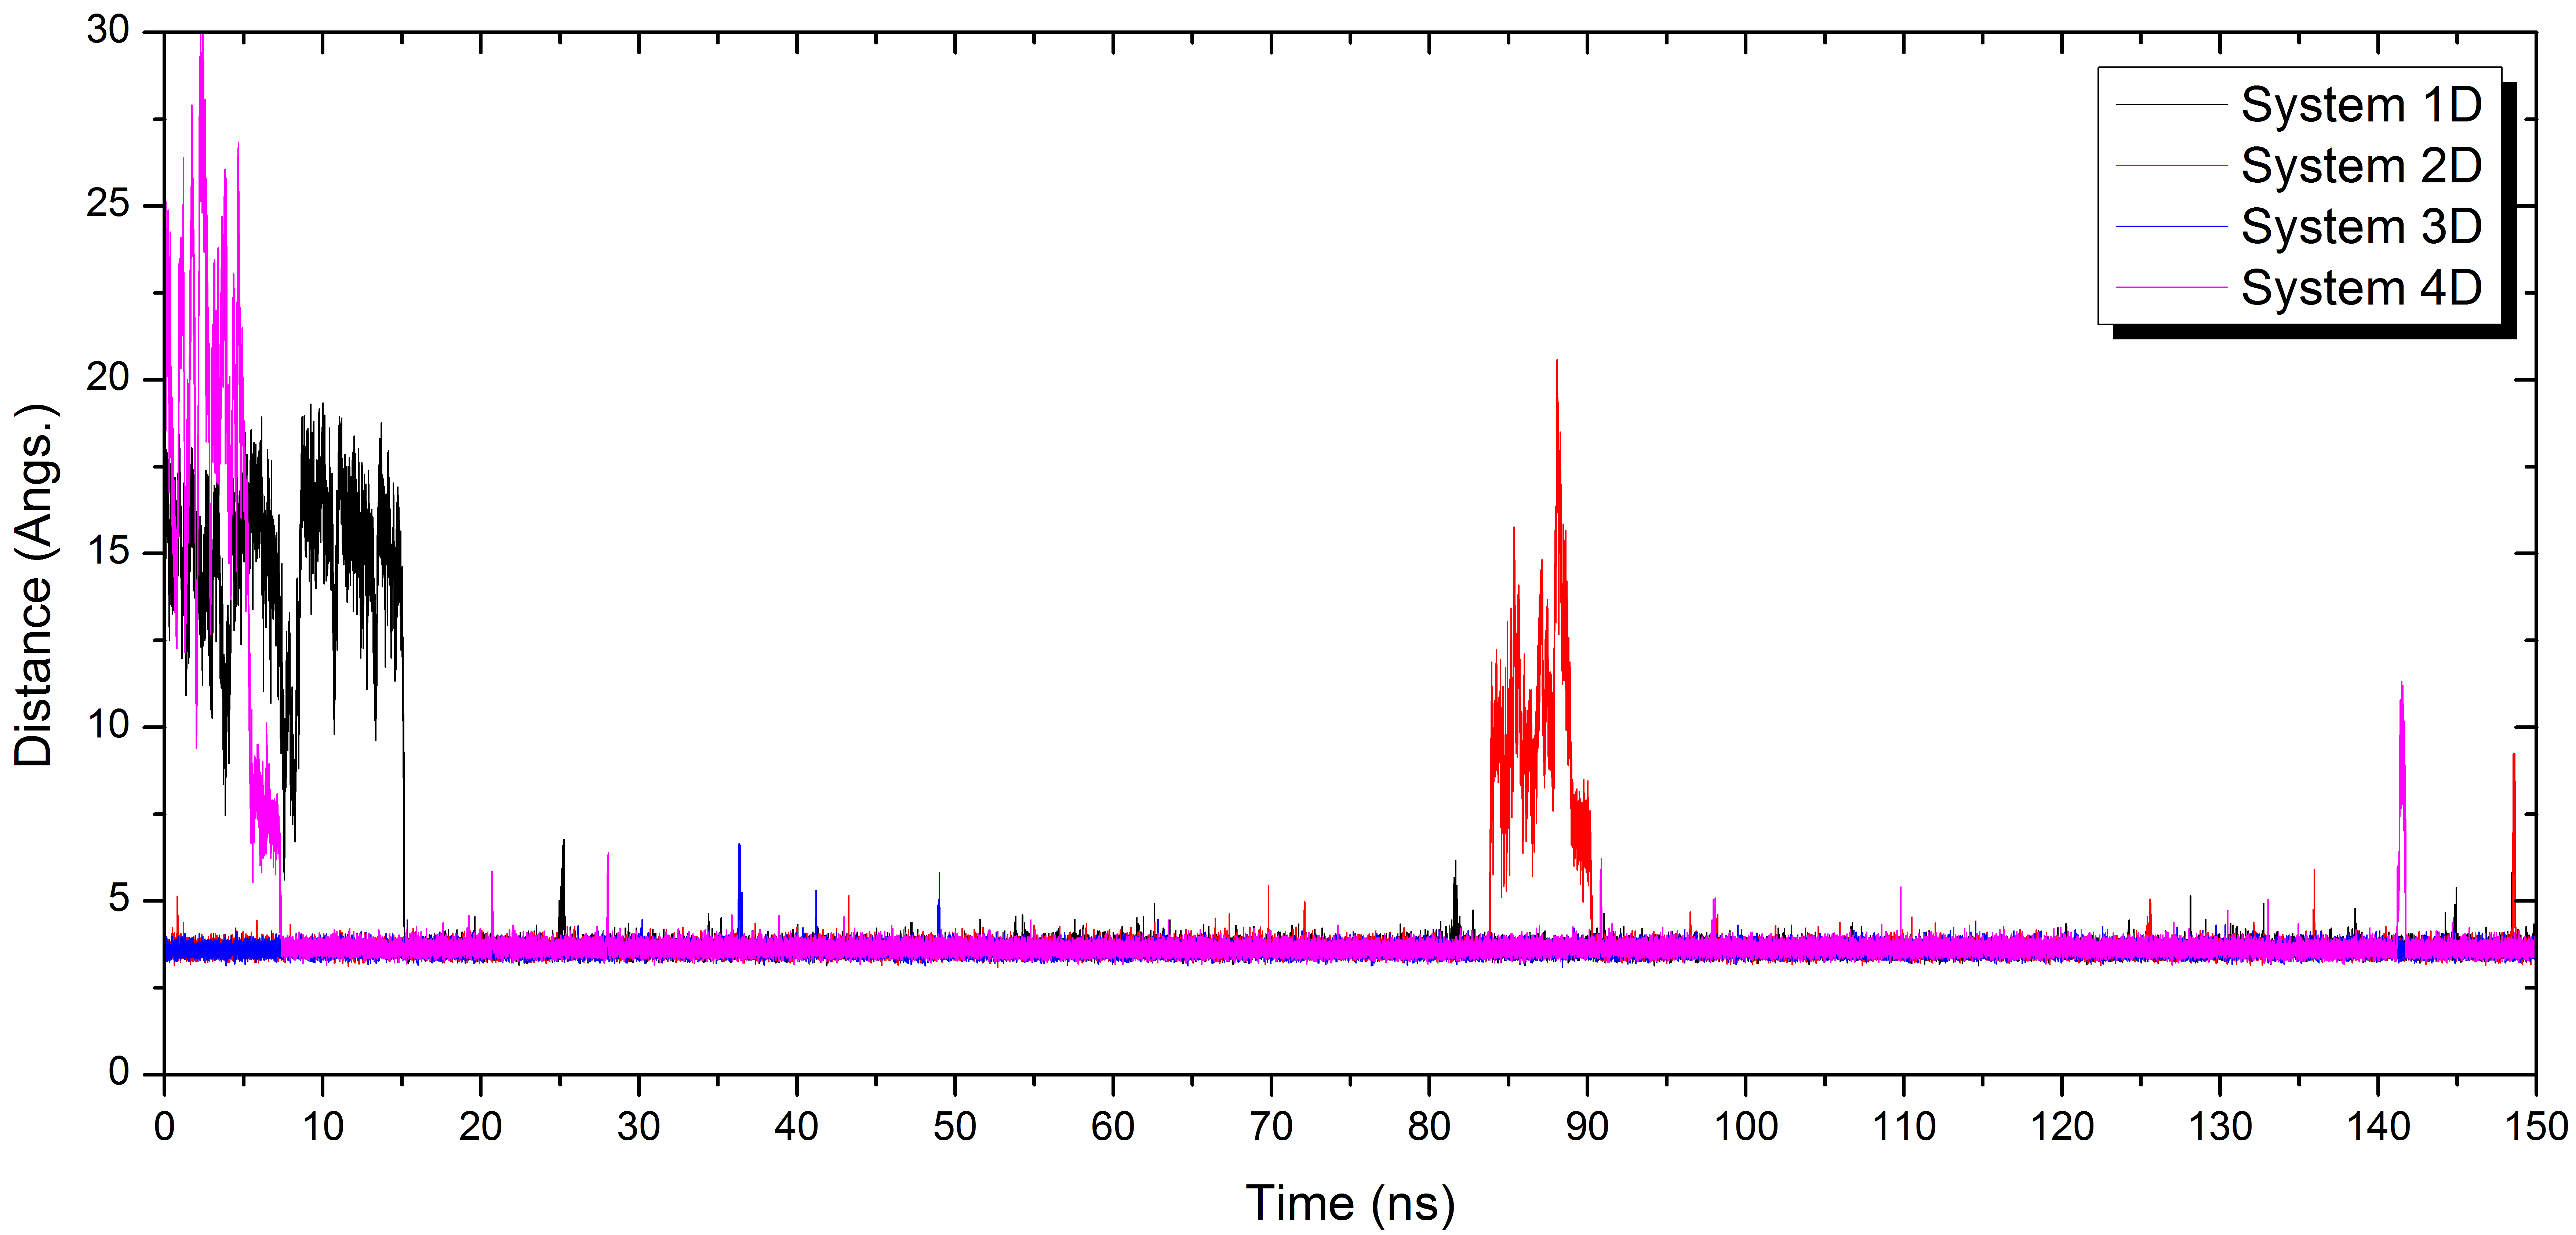
\includegraphics[width=0.45\columnwidth]{image/distance_1-4}&
		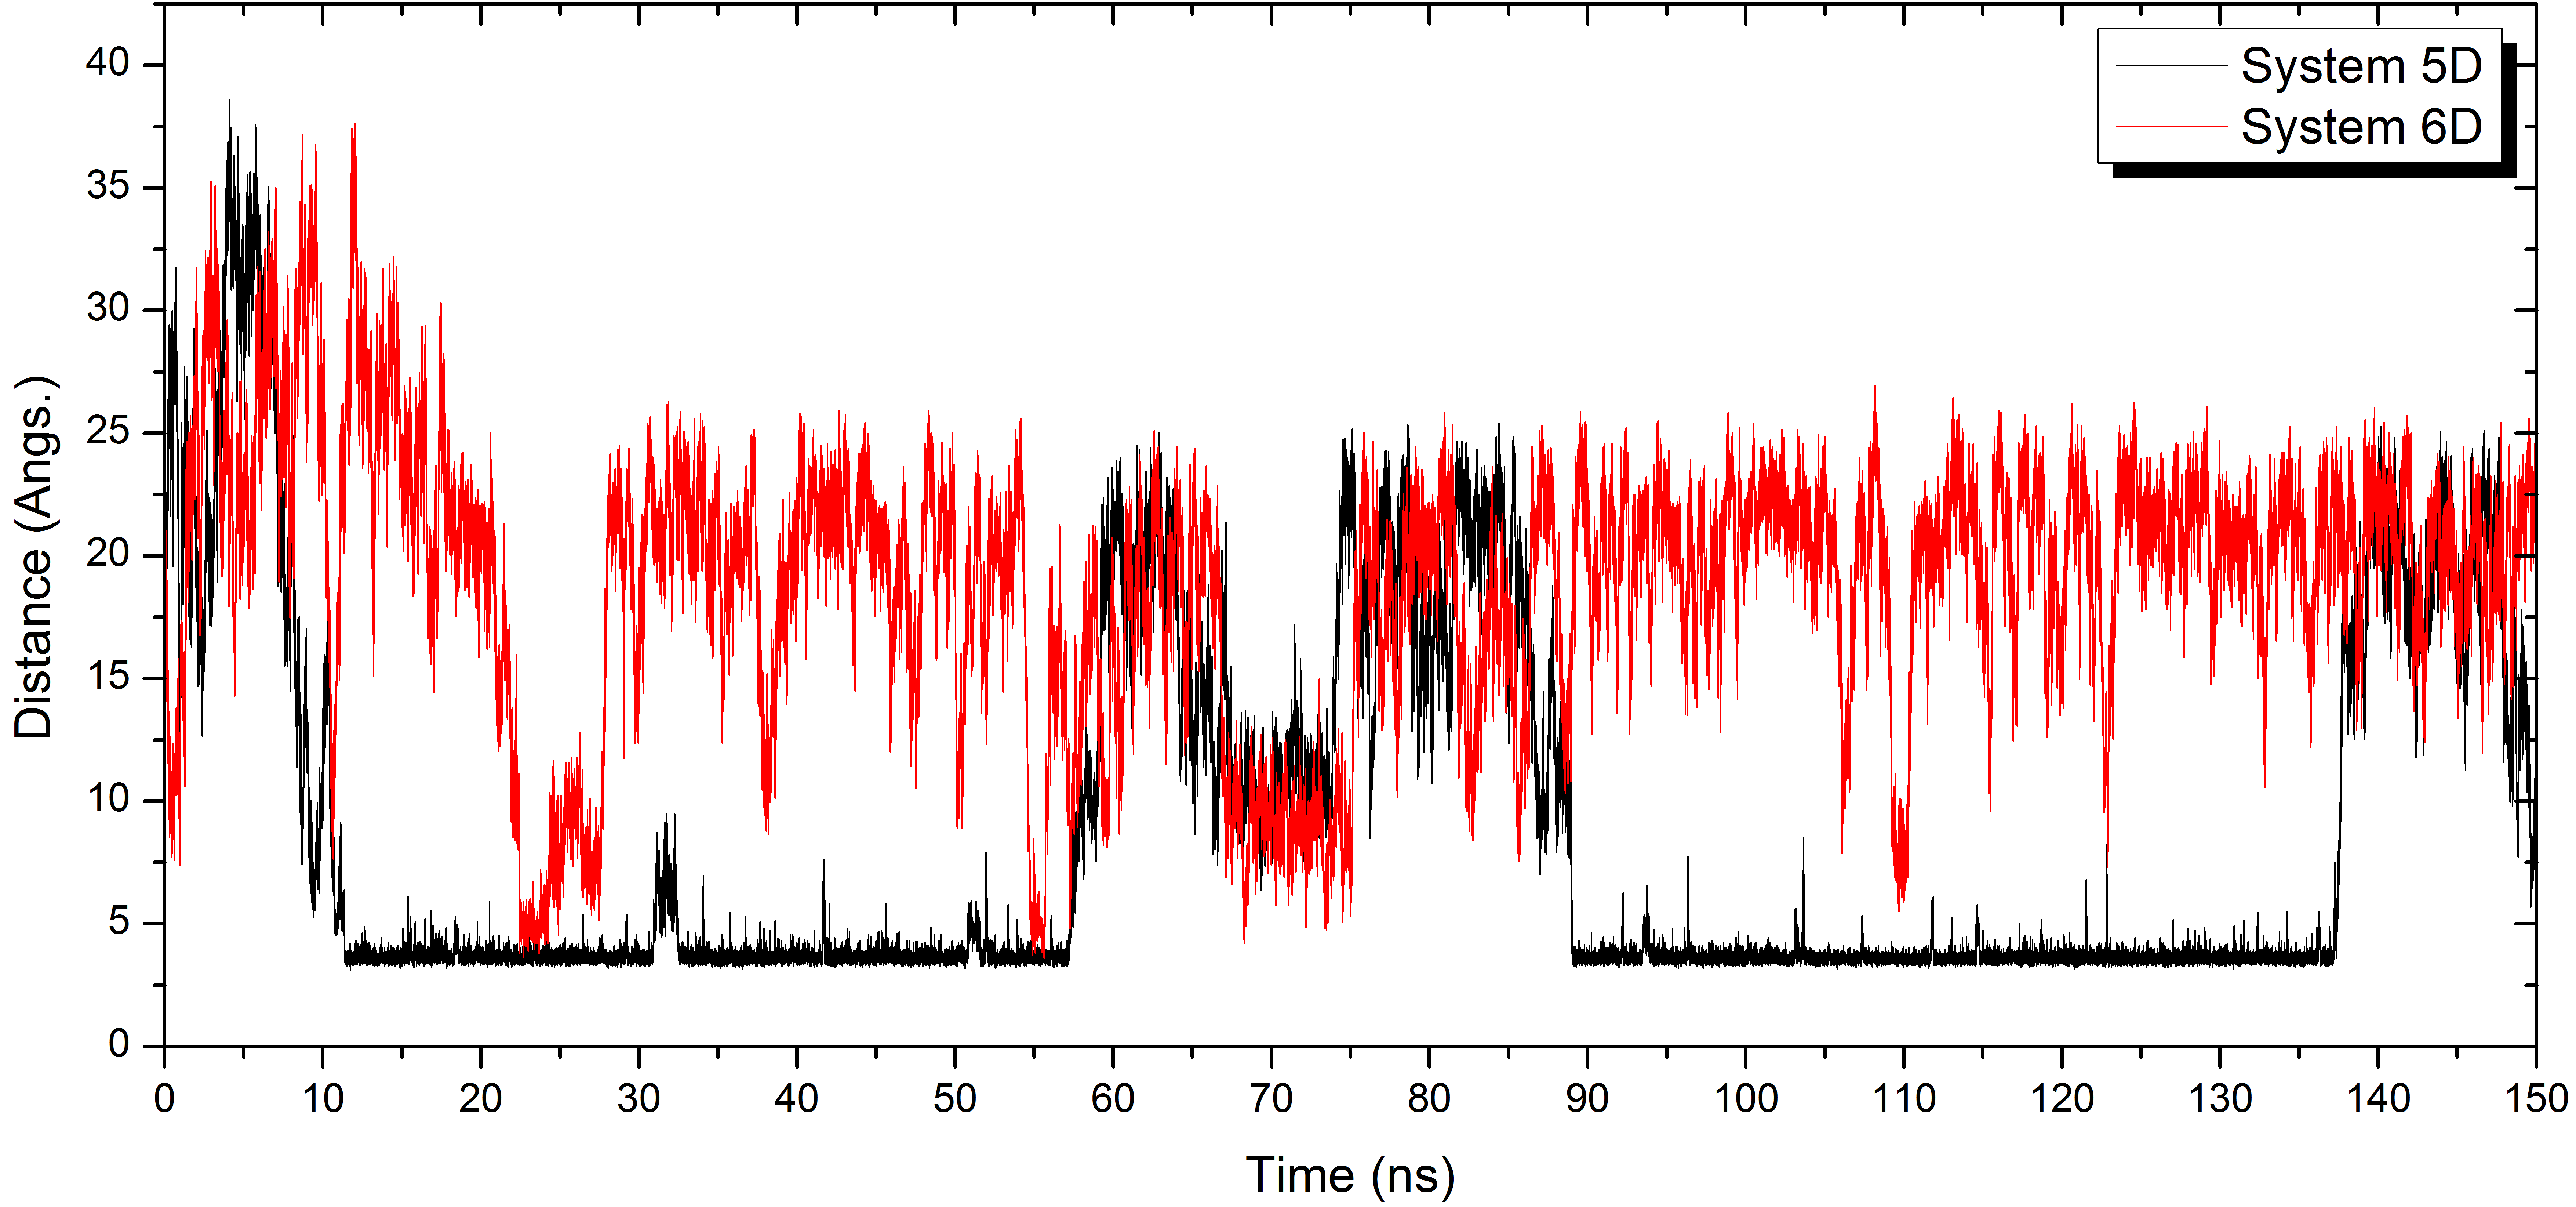
\includegraphics[width=0.45\columnwidth]{image/distance_5-6} \\
	\end{tabular}
	\caption{Distances between monomers for ``random'' starting point.}
	\label{pap:fig08}
\end{figure}

The formation of hydrogen bonds both between two acid chain ends or between an acid chain end and the carbonyl group of the conjugated core are probable to take place for all the 1D-6D systems. One should note that, as it was expected, system 2D has a lower probability of forming such hydrogen bonds interactions because a carbonyl group was replaced by a thionyl one. The same is also true for systems 5D and 6D.\\

The cosine of the angle between the aromatic cores' planes is a useful complementary information towards the determination of the stability of the stack. Values of $\omega = 0^\circ$  (cos $\omega$  = 1) or  $\omega = 180^\circ$ (cos $\omega$ = -1) corresponds to parallel monomers (polyaromatic cores as $\pi-\pi$ stacking), and  $\omega = 90^\circ$ (cos $\omega$ = 0) corresponds to perpendicular molecules (T-shape).\\  

For the ``organized'' starting point, the cosine indicates planar co-facial interacting structures, except for system 1D, which has some fluctuations during the simulation, as it can be seen in Figure \ref{pap:fig09}. For the random starting point, these fluctuations are more common for all the systems in the beginning of the simulation and system 2D has it in the middle of the simulation time. This indicates that, although the parallel co-facial interaction is preferential, as it is also indicated by the minimum distances values, the molecules have some freedom to rotate around their normal axis during the MDS under these thermodynamic conditions. Up to this point, we cannot discern and indicate if this is an effect of the place of the sulfur atom in the structure or if is is just the fact that the hydrogen bonds are dynamic and allow the molecules to rotate. In any case, these results are in agreement with the ones found by Teklebrhan and co-workers.\cite{teklebrhan2012probing} What can be said though is that the 1D-4D systems do not perform T-shape interactions, but this is the case for the system 5D and 6D, as it is reported in Figure \ref{pap:fig10}.

\begin{figure}[p]
	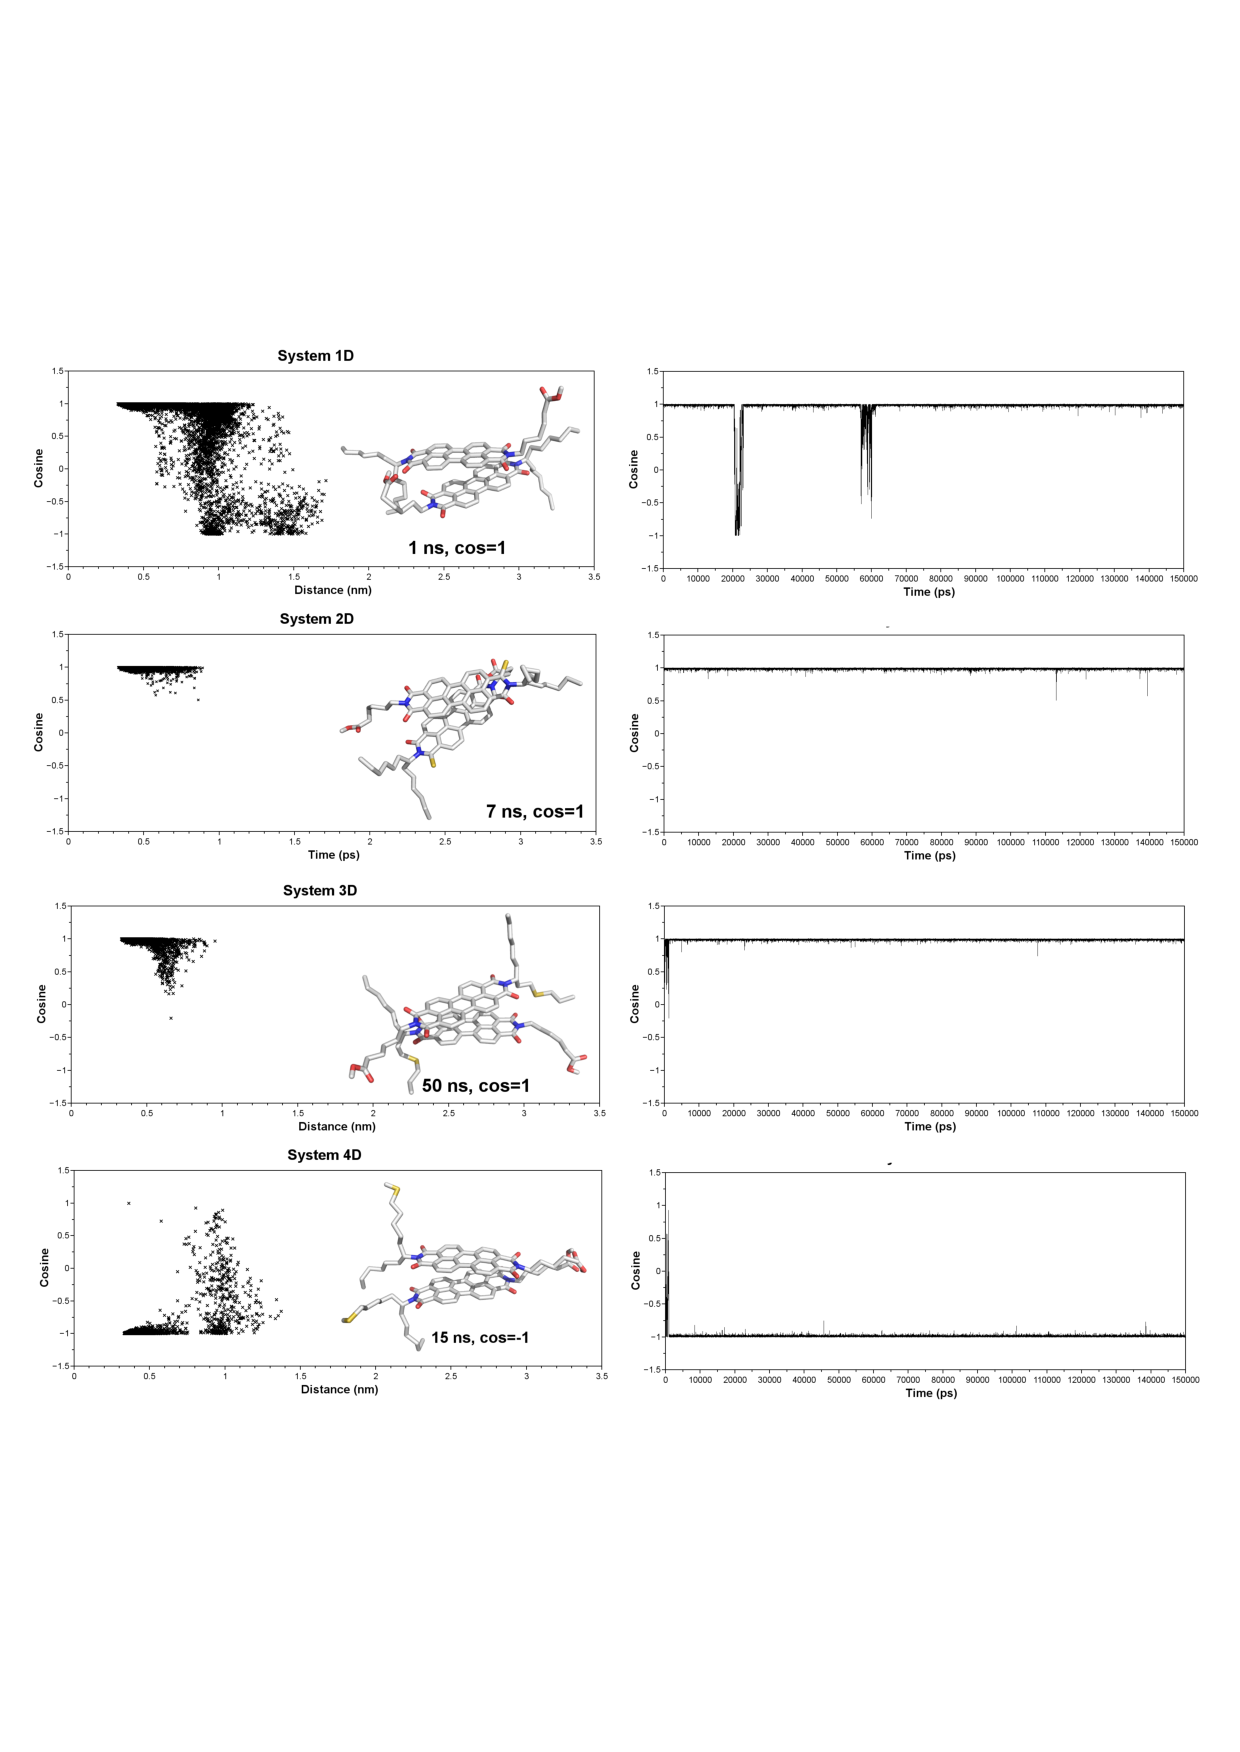
\includegraphics[width=\columnwidth]{image/Figure7}
	\begin{tabular}{cc}
		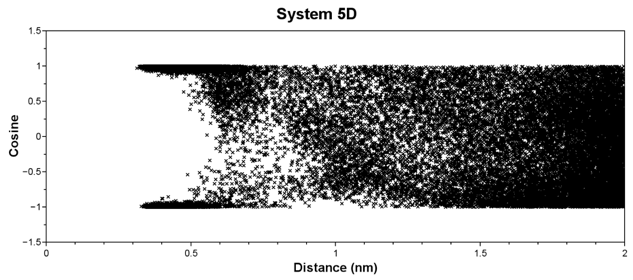
\includegraphics[width=0.45\columnwidth]{image/Figure7b}&
		\includegraphics[width=0.45\columnwidth]{image/Figure7c} \\
	\end{tabular}
	\caption{Cosine of angle between aromatic cores in function of distance between dimers monomers for the organized starting point. Carbon atoms are in grey, oxygen in red, nitrogen in blue and sulfur in yellow. Hydrogen atoms are omitted for clarity.}
	\label{pap:fig09}
\end{figure}

\begin{figure}[htb]
	\begin{tabular}{cc}
		\includegraphics[width=0.45\columnwidth]{image/angle_1-4}&
		\includegraphics[width=0.45\columnwidth]{image/angle_5-6}\\
	\end{tabular}
	\caption{Cosine of angle between aromatic cores in function of distance between dimers monomers for the random starting point. Carbon atoms are in grey, oxygen in red, nitrogen in blue and sulfur in yellow. Hydrogen atoms are omitted for clarity.}
	\label{pap:fig10}
\end{figure}	

The results obtained previously for systems 5D and 6D are now reproduced if the starting configuration is random. System 5D can assume a stable face-to-face configuration during some periods of the simulation but it is not stable throughout it. System 6D is not stable in this configuration and no stable conformation can be noticed by the distances analysis.\\

\textbf{Trimers (Systems 1T - 6T}: Previous molecular dynamics simulations have shown that molecule 1 (C5Pe) has a high tendency to dimerize in toluene, but it does not form larger aggregates, since it has a long and linear alkyl side chains.\cite{teklebrhan2012probing} However, the distance between the monomers of system 1T is constant from the beginning of the simulation, indicating an average height lower than 0.8 nm.  This is in agreement with experimental work,\cite{eyssautier2011insight} which suggest a height of 0.67 nm. Systems 2T and 4T (after 33 ns) exhibit similar results.\\ 

As it can be seen from Figures \ref{pap:fig11}, \ref{pap:fig12}, \ref{pap:fig13} and \ref{pap:fig14}, the fluctuations in these distances are a function of the starting configuration. In ``organized'' starting configuration, system 3T shows larger distances after 45 ns and the molecules are close to each other ($<$ 0.4 nm) at only 4\% of the simulation. For system 3T, the results show variable molecular dissociation of one monomer, but the remaining dimer is stable. For the random starting configurations, systems 1T and 3T are stable as face-to-face aggregates during almost all the simulation time, whereas 2T takes 75 ns to stabilize in this configuration. The 4T now has the same effect in this situation that 3T had before: the trimer is not stable in the face-to-face configuration although the three molecules are kept together by the hydrogen bonds and the two of them assume the face-to-face configuration, as it is the case of 4D system. 

\begin{figure}[htb]
	\centering
	\includegraphics[width=\columnwidth]{image/Figure8} 
	\begin{tabular}{cc}
		\includegraphics[width=0.5\columnwidth]{image/Figure8b} &
		\includegraphics[width=0.5\columnwidth]{image/Figure8c} \\
	\end{tabular}
	\caption{Distances between monomers for ``organized'' starting point.}
	\label{pap:fig11}
\end{figure}

\begin{figure}[htb]
	\centering
	\includegraphics[width=\columnwidth]{image/Figure10} 
	\begin{tabular}{cc}
		\includegraphics[width=0.5\columnwidth]{image/Figure10b} &
		\includegraphics[width=0.5\columnwidth]{image/Figure10c} \\
	\end{tabular}
	\caption{Angle between monomers for ``organized'' starting point.}
	\label{pap:fig12}
\end{figure}

\begin{figure}[htb]
	\centering
	\begin{tabular}{ccc}
		\includegraphics[width=0.3\columnwidth]{image/distance_M1} &
		\includegraphics[width=0.3\columnwidth]{image/distance_M2} &
		\includegraphics[width=0.3\columnwidth]{image/distance_M3} \\
		\includegraphics[width=0.3\columnwidth]{image/distance_M4} &
		\includegraphics[width=0.3\columnwidth]{image/distance_M5} &
		\includegraphics[width=0.3\columnwidth]{image/distance_M6} \\
	\end{tabular}
	\caption{Distances between monomers for ``random'' starting point.}
	\label{pap:fig13}
\end{figure}


\begin{figure}[htb]
	\centering
	\begin{tabular}{cc}
		\includegraphics[width=0.45\columnwidth]{image/angle_M1} &
		\includegraphics[width=0.45\columnwidth]{image/angle_M2} \\
		\includegraphics[width=0.45\columnwidth]{image/angle_M3} &
		\includegraphics[width=0.45\columnwidth]{image/angle_M4} \\
		\includegraphics[width=0.45\columnwidth]{image/angle_M5} &
		\includegraphics[width=0.45\columnwidth]{image/angle_M6} \\
	\end{tabular}
	\caption{Angle between monomers for ``random'' starting point.}
	\label{pap:fig14}
\end{figure}

When the predominant type of interactions was investigated for the case with the ``organized'' starting point, it was noticed they are constant during the whole simulation for system 1T, 2T, and 4T (Figure 9). Those molecules seem to be stable as a trimer. The interaction between the first two aromatic cores is not influenced when a third monomer is added, which in turn, has an identical behavior with the second molecule. It suggests that the interaction driving the aggregation is made from the poly-aromatic cores. Although, the side chain should contribute to aggregation since it interacts during all the simulation for the four systems. 

The monomers geometries can be also analyzed by the cosine values of the angle between poly-aromatic cores (Figures \ref{pap:fig12} and \ref{pap:fig14}). For all trimer systems, the planar configuration is more likely than others, namely the T-shape. System 3T, in the ``organized'' starting point  (Figure \ref{pap:fig12}) and system 4T in the random starting point (Figure \ref{pap:fig14}) show now variations in these angles, either in the beginning or during the whole simulation. This, added to the fact that the intermolecular distance is similar for both 1-3 and 2-3 molecules, is an indication that the dimer is stable and interacts with the third molecule via the hydrogen bonds. 

The distances between monomers of systems indicate greater variation for system 5T and 6T. System 5T shows larger distances after 30 ns and the molecules are close to each other (< 0.4 nm) at only 13\% (19.5 ns) of the simulation. System 5T shows larger distances during the entire simulation, due to monomers dissociation. The trimers geometry was also analyzed by the cosine values of the angle between poly-aromatic cores. For both systems, the cosine does experience large variation and does not have association to short distances.\\ 

The stable trimers also interact through hydrogen bonds during the simulation. On systems 2T, 3T and 4T, the hydrogen bonds interactions occur basically between carboxylic groups of side chains (Figure 11). For systems 4T, the frequency of these hydrogen bonds is higher than 96\% of the total simulation. For systems 3T, the numbers decrease to 63\%, since only side chains from monomers 1 and 2 interact. Furthermore, only for system 1T, the numbers of hydrogen bonds between the side chains and the carbonyl group of poly-aromatic core are significant (80\%). Moreover, the presence of carboxylic acid groups is important to aggregation, but they were not enough present to maintain the trimer in a parallel orientation, as observed in systems 1T, 3T and 4T (from random starting point).

The side chains from trimers interact through hydrogen bonds during the simulation. At systems 5T, the frequency of hydrogen bonds between carboxylic groups of side chains is higher than 50\% (75 ns) of total simulation, but for system 6T, this number decreases to 26\% (39 ns). Moreover, the presence of carboxylic acid group is important to aggregation, but they were not enough to maintain the aggregated in a parallel orientation.\\


\textbf{General effect of the Sulfur atom}: Up to now, the properties of the aggregates of molecules 1-4 has been discussed for dimers and trimers. Although some differences in their dynamics in solution could be noticed during MDS, no final conclusion on the role of the sulfur hetero-element can be extracted so far. In order to circumvent this shortcut, we have introduced, for the random starting configurations, the study of the radial distribution functions (RDF) for the \ce{S-X} pairwise interactions, where \ce{X} can be: 1 - the oxygen atoms of the aromatic core (aromatic carbonyl groups), 2 - the oxygen atoms of the carboxylic acid group (\ce{COOH}), and 3 - the hydrogen atom of the same group. This was motivated since it is known that sulfur atoms can form non-covalent (Coulomb and/or van der Waals) interactions with oxygen and hydrogen,\cite{jackson2013controlling} sometimes strong enough to lock conformations in place. These graphics can be found in Figure \ref{pap:fig16} for the dimer and \ref{pap:fig17} for the trimer systems.\\

\begin{figure}[htb]
	\begin{tabular}{cc}
		\includegraphics[width=0.45\columnwidth]{image/rdf_14} &
		\includegraphics[width=0.45\columnwidth]{image/rdf_56} \\     
	\end{tabular}
	\caption{Normalized Radial Distribution Functions for the trimer systems.}
	\label{pap:fig15}
\end{figure}	

\begin{figure}[htb]
	\begin{tabular}{cc}
		\includegraphics[width=0.45\columnwidth]{image/rdf_SOar} &
		\includegraphics[width=0.45\columnwidth]{image/rdf_SOcarb} \\
		\includegraphics[width=0.45\columnwidth]{image/rdf_SHcarb} & \\        
	\end{tabular}
	\caption{Normalized Radial Distribution Functions for the \ce{S-X} pairwise interactions, where \ce{X} can be the oxygen atom of the aromatic core, the oxygen atom of the carboxylic group (\ce{COOH}) or its hydrogen for the dimer system.}
	\label{pap:fig16}
\end{figure}	


\begin{figure}[htb]
	\begin{tabular}{cc}
		\includegraphics[width=0.45\columnwidth]{image/rdf_SOar2} &
		\includegraphics[width=0.45\columnwidth]{image/rdf_SOcarb2} \\
		\includegraphics[width=0.45\columnwidth]{image/rdf_SHcarb2} & \\        
	\end{tabular}
	\caption{Normalized Radial Distribution Functions for the \ce{S-X} pairwise interactions, where \ce{X} can be the oxygen atom of the aromatic core, the oxygen atom of the carboxylic group (\ce{COOH}) or its hydrogen for the trimer system.}
	\label{pap:fig17}
\end{figure}	

In dimer and trimer systems, all the peaks found in the \ce{S}-aromatic carbonyl oxygen RDFs are due to intra-molecular configurations. This is known by measuring the \ce{S-O} distances of an isolated molecule of each type. Minor peaks, as it is the case of the ones found around 3, 8 and 14 \AA~for system 2D, are due to the interaction with oxygen atoms of the other molecule interacting with the one bearing the reference sulfur atom. The other systems show similar behavior with wider peaks now due to the fact that sulfur atoms are in flexible parts of the molecule. This allows us to state that there is no particular affinity between sulfur atoms and aromatic carbonyl atoms in the studied structures and this cannot be a likely interaction mechanism.\\

The \ce{S-O} (\ce{COOH}) and \ce{S-H} have now new features that could not be observed in the previous case. Considering both dimer and trimer systems, these two RDFs have intra-molecular peaks centered at around 18 \AA~for molecule 2 (systems 2D and 2T), 22 \AA~for molecule 3 (systems 3D and 3T), and 26 \AA~for molecule 4 (systems 4D and 4T - out of the measurement range, but one can see the peak in the end of the graph). The other peaks are due to inter-molecular interactions between adjacent molecules. Molecule 2, regardless if it is a dimer or a trimer, does not have these additional peaks, indicating that the presence of the sulfur atom on the conjugated backbone does not have any particular affinity with neither oxygen or polar hydrogen atoms of the other molecules. On the other hand, molecule 3 (system 3D) has a ``bump'' for both \ce{S-O} (\ce{COOH}) and \ce{S-H} (\ce{COOH}) RDFs centered at 8 \AA~that does not come from an intra-molecular interaction and is a signature of inter-molecular affinity between the sulfur atom and these oxygen and hydrogen atoms. This behavior is more pronounced in trimer systems, as it expected, since this interaction can take place more easily.\\

This behavior is still more pronounced for molecule 4 (system 4D and 4T): the \ce{S-O} and \ce{S-H} inter-molecular interactions are now very likely to take place and, considering the peak centered in 2.5 \AA~of the S-H RDF that is not present in the \ce{S-O} curve (see Figure \ref{pap:fig09}), one could say that there is also an affinity of this terminal \ce{-SH} group with the acid chain ends of the neighbor molecule. This same characteristic is found for trimer systems (Figure \ref{pap:fig10}).\\

Based on these observations, one can state that sulfur atoms grafted directly to the conjugated backbone has a little influence on the dynamic behavior of dimer and trimer asphaltene systems and one might not be able to differentiate this with what is observed for the case where there is no sulfur atom (molecule 1). Oppositely, the presence of sulfur atoms on the lateral chains, either in the middle of it or as a chain end, has a more pronounced effect on the properties of these molecules (molecules 3 and 4). This is due to the fact that this atom can now interact with acid chain ends of neighbor molecules by means of non-covalent interactions like Coulomb and/or van der Waals.\\

Although the differences herein highlighted can, in our scale, not be of uppermost importance, it is the case in oil industry where huge quantities of molecules are being treated at the same time. These results can help towards the comprehension why crude oils with an elevated sulfur content are more difficult to crack, as a matter of fact. 


\clearpage

\subsection{Schuler's-derivatives systems}

The systems were arranged so that to determine the separated effects of the different heteroatoms and the chain-ends.

\subsubsection{Effect of the heteroatom}

In order to study the effect of the heteroatom on the aggregation process of the PA3-type molecule, we screened the three free positions letting \ce{X} assume the values of \ce{O}, \ce{S} and \ce{NH}. Moreover, the chain-end for this purpose was chosen to be \ce{-CH3} in order to avoid any effect due to hydrogen-bonding on the aggregation mechanism, as it will be studied later on. Thus, the following systems were considered: A13, A23, A33, A43, and A53. Although only one heteroatom is found in family CA22, \textit{i.e.} nitrogen, we also present here, for the sake of comparison, the results obtained for the AAC molecule. In Figure \ref{pap:fig18}, one can find the normalized RDF functions  of these systems under 298 K and 1 bar conditions.

\begin{figure}[h]
	\begin{tabular}{cc}
		\includegraphics[width=0.45\columnwidth]{image/02a} & 	
		\includegraphics[width=0.45\columnwidth]{image/02b} \\
		(a) & (b) \\
	\end{tabular}
	\caption{Aggregation mechanism with \ce{-CH3} ended chains: (a) effect of the heteroatom (A13, A23, A33, A43, A53)  and (b) effect of the asphaltene type (A53/AAC). Each peak of the RDFs corresponds to a neighbor molecule in the $\pi$-stacking structure presented in Figure \ref{pap:fig03}.}
	\label{pap:fig18}
\end{figure}

These curves describe the organization structure in liquid state of the asphaltene solution. Such regular separation between peaks with an interval of around 3.9 \textup{\AA} indicates that the asphaltenes are organized in a stack structure. The first peak centered at $\sim$ 3.9 \textup{\AA} stands for the interactions with the first neighbors generated by the $\pi$-stacking interaction. Depending on the position of the molecule within the stack, it can have one or two first neighbors. The other peaks represent the second, third and fourth neighbors in the stack. In this way, as the RDFs describe a probability density, it is almost twice more probable for an asphaltene to have a first neighbor at 3.9 \AA~than a second neighbor at 7.8\AA.\\ 

Different heteroatom substitution has a slight effect on the shape of the RDFs, although there are intensity changes (not seen here because the normalized version is presented). This is probably due to the fact that the total density of the liquid is slightly changed in function of the heteroatom (as they have different masses and different Van der Waals radii). The most important change concerns the CA22 asphaltene type AAC. This molecule has an aggregation pattern that also follows a stack architecture but high-order neighbors are not as probable as they are for the PA3 type. This is indicative of a short-range order whereas a long-range one is not kept during the simulation. This is evidenced by the snapshots of their molecular architecture after 60 ns of molecular dynamics simulation at 298K and 1 bar in Figure \ref{pap:fig19}.

\begin{figure}[h]
	\begin{tabular}{cc}
		\includegraphics[width=0.45\columnwidth]{image/A33_60ns} & 	
		\includegraphics[width=0.45\columnwidth]{image/AAC_60ns} \\
		(a) & (b) \\
	\end{tabular}
	\caption{60 ns-snapshots of 5 molecules of each asphaltene in toluene at 298K and 1 bar conditions: (a) A33 and (b) AAC. Carbon atoms are presented in gray and nitrogen atoms in blue. Aromatic or polar hydrogen atoms are presented in white. Toluene molecules are omitted for clarity.}
	\label{pap:fig19}
\end{figure}

Whereas PA3-type molecules, regardless of the heteroatom, aggregate forming co-facial planes, CA22-type molecules stack in a not completely planar way, leaving room to the formation of tilted architectures between adjacent molecules. This is the case during the whole simulation. This explains the lower intensity peaks present in the RDF. In order to deeply understand these features, the analysis of the energies of interaction is then a powerful tool to elucidate the effect of changing the heteroatom on the aggregation strength of these molecules. We studied the dimers of each molecule in vacuum dynamics for 10 ns using the same conditions as during the stabilization step. The time-averaged interaction energy $<E_i>$ was determined by:  

\begin{equation}
<E_i>=-(<E^p_d> - 2.<E^p_m>)
\end{equation}

$<E^p_d>$ stands for the average value of the potential energy of the dimers after it has stabilized and $<E^p_m>$ is the average value of the potential energy of a single isolated molecule after it has stabilized. The same method of calculation has been used by Liu \textit{et al.}\cite{liu2015molecular} The interaction energies of PA3 and CA22 dimers in vacuum, reported in Table \ref{pap:tab02} (diagonal values), corroborate the interpretation extracted from the analysis of the RDF functions: for any given molecular structure within the same class, changing one heteroatom by another has a slight effect on these molecules' dimers aggregation. The energies of interaction fluctuate around the average value of 55.7 kcal.mol$^{-1}$ (3.8x10$^{-19}$J) for the PA3 class of molecules. For the CA22 molecule type, the interaction energy is lowered by around 10 kcal.mol$^{-1}$. The out-of-diagonal values reported in this Table will be discussed in the next sections.

\begin{table}[h]
	\centering
	\begin{tabular}{c|cccccc}
		\hline
		& A13 & A23 & A33 & A43 & A53 & AAC \\
		\hline         
		A13 & 56.2 & 40.9 & 37.4 & - & - & 42.2 \\        
		A23 & 40.9 & 52.2 & 46.7 & - & - & 47.4 \\
		A33 & 37.4 & 46.7 & 57.0 & - & - & 35.2 \\
		A43 & - & - & - & 58.9 & - & - \\
		A53 & - & - & - & - & 54.0 & - \\
		AAC & 42.2 & 47.4 & 35.2 & - & - & 45.8 \\
		\hline
	\end{tabular}
	\caption{Interaction energies ($<E_i>$) in kcal.mol$^{-1}$ calculated for PA3- and CA22-type dimer molecules.}
	\label{pap:tab02}
\end{table}

One should keep in mind that these molecules present different contributions of the Van der Waals and the Coulomb terms to the potential energy. Whereas one should expect the Van der Waals energy term to be higher for molecules containing Sulfur atoms than molecules containing Nitrogen and Oxygen atoms (motivated by the increase of the C$_6$ and C$_{12}$ Van der Waals terms, respectively). On the contrary, the Coulomb terms involving Oxygen should be higher than Sulfur's and Nitrogen's, motivated by the increased local dipole moments. In this way, the interaction energies result of both effects taking place at the same time, besides other contributions due to the angle, dihedral and improper torsion terms that are not equivalent elsewhere. The Van der Waals interactions are understood as the combination between Lennard-Jones repulsion terms (with a $r^{-12}$ dependence) and the London dispersion/attractive terms, which is originated from induced dipole-induced dipole interactions (with a $-r^{-6}$ dependence). Finally, it is worth noting that the Coulomb interactions, besides having a repulsive/attractive $r^{-1}$ character, occur between fixed dipoles/charges-fixed dipoles/charges.\\

Decomposing the total potential energy in these terms, we found that the highest contribution to the interaction energy comes from the non-bonding Van der Waals potential terms. These contributions represent 86, 81, 84, 85, 82 and 73 \% of the total interaction energy for A13/A13 ... AAC/AAC interaction pairs, respectively. The Coulomb energy contributions are not higher than 4\%. This result indicates that, for the situations where a molecule interacts with a similar one, the Van der Waals forces govern the aggregation between the adjacent molecules. 

\subsubsection{Effect of chain-end}

Having such results in mind, we studied the presence of \ce{-COOH} functions on the chain-ends for the same molecules under the same conditions, for A11, A21, A31, A41, A51 and AAA. Molecules A12 and AAB are presented in a separate plot that can be found in the ESI. The normalized RDF functions for these systems can be found in Figure \ref{pap:fig20}.

\begin{figure}[h]
	\begin{tabular}{cc}
		\includegraphics[width=0.45\columnwidth]{image/04a} & 	
		\includegraphics[width=0.45\columnwidth]{image/04b} \\
		(a) & (b) \\
	\end{tabular}
	\caption{Aggregation mechanism with \ce{-COOH} ended chains: (a) effect of the heteroatom (A11, A21, A31, A41, A51)  and (b) effect of the asphaltene type (A51/AAA). Each peak of the RDFs corresponds to a neighbor molecule in the $\pi$-stacking structure presented in Figure \ref{pap:fig19}.}
	\label{pap:fig20}
\end{figure}

The RDFs differ significantly from the previous case with no acid chain: they are characteristic of liquids where the aggregates concern the stack of only two molecules, longer stacks presenting a lower probability. The interactions are now governed by another mechanism and the structure of the aggregate is less ordered in comparison to the stack structure, probably due to the presence of H-bonds, which signature can be seen as the 2 \textup{\AA} small peaks. The acid chain-ends have an effect of overwhelming the $\pi$-stacking interactions beyond the second neighbor, hiding the third- and fourth-neighbor peaks.\\

The loss of symmetry due to the formation of H-bonds is identified in the RDFs by the wide peaks appearing for lengths superior to 10 \textup{\AA}. This wide peak is attributed to the interaction between asphaltene aggregates that are not rigid and have gained degrees of freedom from the presence of the H-bonds. Moreover, these wide poorly-defined bands can hide underneath it the peaks due to $\pi$-stacking aggregation. This can be visualized in the snapshots of A31, AAA, A33 and AAC presented in Figures \ref{pap:fig19} and \ref{pap:fig21}.

\begin{figure}[h]
	\begin{tabular}{cc}
		\includegraphics[width=0.5\columnwidth]{image/A31_60ns} & 	
		\includegraphics[width=0.5\columnwidth]{image/AAA_60ns} \\
		(a) & (b) \\
	\end{tabular}
	\caption{60 ns-snapshots of 5 molecules of each asphaltene in toluene at 298K and 1 bar conditions: (a) A31 and (b) AAA.}
	\label{pap:fig21}
\end{figure}

Interestingly, the formation of H-bonds are stable enough under these conditions to avoid the self-stacking as it is the case of the \ce{-CH3}-ended molecules. This characterizes the formation of an elongated cluster in the presence of more than five molecules and could also be responsible for forming larger clusters more rapidly. The interaction energy of two $n$-hexanoic acid chains alone was calculated under the same conditions as before and we have found it to be as high as 22 kcal.mol$^{-1}$ for each pair of \ce{-COOH} groups. When decomposed, this energy is consisted of a balance between the Coulomb and Van der Waals interactions. The intensity of the binding character of Coulomb interaction is around 10 times bigger than the repulsion character of Van der Waals interaction.\\ 

This result shows that the presence of acid chain-ends and the consequent formation of H-bonds within the crude oil is also a great aggregation factor. This can explain why these molecules are so difficult to treat in oil industry's production chain. Total interaction energies can be estimated to be as high as 75 kcal.mol$^{-1}$, including both the $\pi-\pi$ and a pair of H-bond interactions, as aforementioned. Such a strong interaction between two adjacent molecules is almost equivalent to a covalent bond. For larger aggregates, this energy should be multiplied by the number of aromatic cores in interaction and the total number of acid chain-ends.\\

As it has been reported experimentally,\cite{durand2010effect} the macro-aggregates should be linked to each other by weak dispersive interactions between their lateral chains or simply because they are more polar than their environment, causing that they remain close together. This should explain why, experimentally, stirring the sample is enough to separate these aggregates in smaller pieces. In an underneath scale, the interactions should be governed by H-bonds which are much more robust and should keep the nano- and/or micro-aggregates in place. Finally, the same H-bonds and the $\pi$-stacking between the conjugated planes as herein studied are supposed to be the interactions ruling the aggregation phenomena at the nano-scale. This multi-scale model of the organization of asphaltene aggregates was first proposed by Mullins \textit{et al.}\cite{mullins2010modified,mullins2011asphaltenes,mullins2012advances}

\subsubsection{Aggregation within heterogeneous boxes}

Next, we will present the results of aggregation for boxes containing different asphaltenes, be it the same family or not. For the simulation of the mixtures between asphaltenes of the same family, we continued on using the same conditions but varied the relative concentration between the constituents.\\

As it was aforementioned, the effect of the heteroatom on the asphaltene aggregation with a given family can be considered as important as the difference of energies between two different classes of them. This means that, the effect of the heteroatom cannot be, at this point, ignored since the difference in energy found when changing it with a the same family of molecules (say A13 and 133) is of the same order of magnitude of the energy difference found when the asphaltene family is changed (say A13 and AAC). But, as a single model cannot be formulated to capture the effect of all the possible combination of heteroatoms, we excluded from now on the structures containing two different heteroatoms on the conjugated core of the same molecule (A41, A43, A51 and A53). This allows us to still have a large variety of possible combinations.\\

Firstly, we study the binary mixtures within the PA3 molecular family. The combinations were done in order to screen the effect of relative concentration keeping constant the total number of five molecules within the simulation box. The concentrations were screened replacing a molecule of one type of asphaltene by another one at a time. This scheme is better understood after seeing Table S2 in the ESI (Mix 1a to 1d).

The simulation of these systems produces two different RDFs: the self-interaction and the cross-interaction curves. The first one describes the probability of any given molecule to interact with a system of the same nature during the simulation and the second one describes the probability of interaction between two different molecules. The curves for the A13:A23 mixture are presented in Figure \ref{pap:fig22}. A13:A33 and A23:A33 mixtures can be found in Figure S1. 

\begin{figure}[htb]
	\centering
	\includegraphics[width=0.4\columnwidth]{image/06a} 
	\caption{Effect of the mixture of A13 and A23 asphaltene molecules with \ce{-CH3} lateral chain-end. This mixture concerns different ratios between Oxygen and Sulfur in the nano-aggregate.}
	\label{pap:fig22}
\end{figure}

These curves indicate that, regardless of the heteroatom, the asphaltenes have similar aggregation mechanisms, \textit{i.e.}, the self-aggregate forming $\pi$-stacks with equidistant separation. This is represented by the peaks in the RDFs. As a matter of fact, A13 has the same interaction pattern with itself regardless of the concentration of A23 and the same is also valid for A23. This is an indicative that the presence of an asphaltene containing a different heteroatom on the backbone does not interfere on the aggregation of the parent molecule. Furthermore, the fact that not all the peaks are present for a given pair of molecules, e.g. A13-A13, indicates that the reference molecule has no similar to it as a first neighbor but it does have one as a second neighbor, what means that the asphaltenes are randomly intercalated among each others. Similarly, when the reference is A13, for instance, the probability of having A23 neighbors increases with the increase of A23 concentration, as it is expected. These very same conclusions can also be found for the other mixtures, concerning oxygen and nitrogen and sulfur and nitrogen ones.  This allows one to say that, on the basis of these results, the aggregates formation is similar regardless of the combination among the heteroatoms. The major differences in these curves are originated from the random intercalation of the different molecules in the formation of the stack. 

As previously, in order to discriminate if there is indeed any difference in the nano-aggregation process, the energies of interaction between each different asphaltene were studied and they are presented in Table \ref{pap:tab02} (off-diagonal values). It can be seen that the pairwise interaction energy changes for different combination of asphaltenes, \textit{i.e.}, every molecule interacts more strongly with an identical molecule than with a different molecule. This effect might be directly associated to the Coulomb and Van der Waals interactions between these molecules. Upon mixing, the Van der Waals energies are expected to reduce. This is a consequence of the combination rule used to determine the Van der Waals coefficients \ce{C6} and \ce{C12} of two distinct $i,j$ atom pair ($C^{6,12}_{ij}=\sqrt{C^{6,12}_i \times C^{6,12}_j}$) induces that the cross-interactions coefficients to be smaller than the original ones. 

\section{Conclusions}

Several asphaltene structural models have been proposed in the literature, such as the C5Pe molecule. Based on experimental work of Eyssautier and co-workers,\cite{eyssautier2011insight} we have chosen six different model molecules for investigating the role of the sulfur atom position within the asphaltene structure. The molecular dynamics simulations have allowed understanding the stability of asphaltene dimers and trimers in toluene as well as showing that the position of the sulfur atom has an effect on the intermolecular non-covalent interactions that can take place in these systems.\\ 

Although the polar side chain is important for determining the aggregation, the main interactions between the molecules are produced by the poly-aromatic cores, which are responsible to the parallel orientation of molecules. This geometry is confirmed by the cosine of angles between the poly-aromatic cores. 
We suggest that the presence of one sulfur atom in the poly-aromatic core (molecule 2) do not prevent the aggregation, since systems 2D and 2T are stable and the radial distribution functions of the pairwise interaction of this atom and the oxygen atoms of the neighborhood do not show any particular affinity. However, the presence of four sulfur atoms in poly-aromatic core avoids the molecules aggregation in a major part of the simulation and this may be due to both steric hindrance, Coulomb repulsion between sulfur and nitrogen atom of the adjacent molecule. Moreover, this molecular structure can not form hydrogen bonds between the acid chain end and the conjugated core of the molecule. On the other hand, sulfur atoms in the middle of the aliphatic chain, as well as a chain end, have a measurable effect on the stability of both dimers and trimers and this is due to the fact that they have a low, still measurable, interaction with the acid chain end oxygen and hydrogen atoms. Finally, these results can help towards the comprehension why heavy crude oils containing high values of sulfur are experimentally more difficult to treat and to crack.\\

Secondly, we have also studied the effect of mixing different asphaltene molecules on their nano-aggregation and which screening was based on experimentally isolated and identified molecules by Schuler and co-workers.\cite{schuler2015unraveling} Molecular dynamics simulations were used in order to identify the nano-aggregation in homogeneous, heterogeneous and \textit{super}-heterogeneous boxes. The first one consisted of only a type of asphaltene at a time; the second one had, within the same class, different asphaltenes mixed for different concentrations varying the heteroatom and the presence of acid chain-ends; and the third type included the mixing of asphaltenes of different classes with variation of the relative concentration. It seems that the nano-aggregation of these molecules is dependent on the heteroatom on the conjugated core and is more dependent on the chain-end and conjugated core size. The energies of interaction for each mix were calculated and are of the same order of magnitude. However, the energy of interaction between the same type of asphaltene tends to be always higher than the energies between different types and/or classes of molecules. The contribution of the acid lateral chains to the interaction energy was calculated and found to be as high as 22 kcal.mol$^{-1}$. Moreover, changing the heteroatom can induce changes up to 10\% of the total interaction energy if compared to other heteroatom. Finally, one should conclude that the aggregation mechanism might be much more strongly correlated to the size of the conjugated aromatic core and the size and nature of lateral chains than the presence of a particular heteroatom. These results are of great importance to oil industry and can help understanding how the molecular cartography of asphaltene molecules can induce stronger interactions or not. 